% \documentclass[a4paper]{report}
% \documentclass[a4paper]{scrreprt}
\documentclass[
    a4paper,     % DinA4 Papier
    11pt,        % Schriftgröße
    twoside,     % oneside, twoside
]{report}

%!TEX root = ../main.tex


%advice: in linux, put new style files into something like /usr/share/texmf/tex/latex and then run ``texhash''


% \usepackage{newclude}	% for the option \include*{...}, to prevent pagebreak between consecutive sections saved in two different files. (reimplementation of \include and \includeonly -> http://www.ctan.org/pkg/newclude)


\usepackage{caption}
\usepackage{lineno}	% allows line numbering: \linenumbers
\usepackage{setspace}	% allows line spacing: \singlespacing,\onehalfspacing,\doublespacing
\usepackage{graphicx}
\usepackage{color}
\usepackage{makeidx}
\usepackage{fancyhdr}	%options for headers and footers
\usepackage[pagebackref=true,plainpages=false,pdfpagelabels]{hyperref}
\usepackage[ngerman,english]{babel}
\usepackage{mathtools}%extention to amsmath; loads amsmath; 
\usepackage{xspace}% when used in newcommand, space is only inserted, if not followed by dot, comma... Must be written at the LAST spot within the braces of a newcommand!!!
\usepackage{parskip}
\usepackage{subcaption}% use this package if subfigures are wanted, contains newest implementation of subfigures
% \usepackage{cleveref}%supports cref to reference multiple things in a row and to automatically write into the text what object is referenced to(http://get-software.net/macros/latex/contrib/cleveref/cleveref.pdf)
\usepackage[plain]{fancyref}%usage: \autoref{type:title} or \autoref{type:title}, gets information about kind of referenced stuff and writes name&number
\usepackage{textcomp}
\usepackage{gensymb}%for units
\usepackage{siunitx}
% \usepackage{showlabels}
% \usepackage{showframe}

% \usepackage{booktabs}

\usepackage{backref}

\usepackage[showframe, headheight=14pt, margin=2.2cm,includehead,includefoot]{geometry}% Set margin sizes, put in showframe to show the frames on document
\geometry{bindingoffset=1cm}

\usepackage{todonotes}

\hypersetup{%
  pdftitle=PhD Thesis,
  pdfauthor=Sarah Lindner,
  colorlinks=false}

% \setlength{\headheight}{13.7pt}%make the header size higher (e.g. if superscripts used in header)

\DeclareGraphicsExtensions{.eps}

% \pagestyle{fancy}

%\usepackage[nomarkers,nofiglist,figuresonly]{endfloat} %put all figures to the end of document


%!TEX root = ../main.tex

%physics commands


%text commands--------------------------------------------------------------------------------
% to get the plural form without a space between the word and s, type {} between the command and s, e.g. \velo{}s -> Vertex Locators


%----------General------------------
\newcommand{\MC}{Monte Carlo\xspace}
\newcommand*{\bg}{background\xspace}
\newcommand{\SM}{Standard Model\xspace}

%---------Setup---------------------------
\newcommand{\na}{numerical aperture\xspace}
\newcommand{\hbt}{Hanbury Brown and Twiss\xspace}
\newcommand{\apd}{avalanche photo diode\xspace}
\newcommand{\cw}{continuous wave\xspace}
\newcommand{\smf}{single mode fiber\xspace}
\newcommand{\vcsel}{vertical-cavity surface emitting laser\xspace}


%-----------Quantum optics---------------
\newcommand{\zpl}{zero-phonon-line\xspace}
\newcommand{\Zpl}{Zero-phonon-line\xspace}
\newcommand{\ZPL}{zero-phonon-line\xspace}
\newcommand{\pl}{photoluminescence\xspace}
\newcommand{\cwl}{center wavelength\xspace}
\newcommand{\lw}{linewidth\xspace}
\newcommand{\gt}{\ensuremath{g^{(2)}}\xspace}
\newcommand{\gtz}{\ensuremath{g^{(2)}(0)}\xspace}


%-----------Diamond material---------------
\newcommand{\nd}{nanodiamond}
\newcommand{\nds}{nanodiamonds}
\newcommand{\Nd}{Nanodiamond}
\newcommand{\basd}{bead-assisted sonic disintegration\xspace}
\newcommand{\cvd}{chemical vapor deposition\xspace}
\newcommand{\hpht}{high-pressure high-temperature\xspace}


%----------Color Center--------------------
\newcommand{\sivc}{silicon-vacancy center\xspace}
\newcommand{\siv}{SiV center\xspace}
\newcommand{\nv}{NV center\xspace}
\newcommand{\sivs}{SiV centers\xspace}

%-------Elements---------------------
\renewcommand{\si}{silicon\xspace}
\newcommand{\ir}{iridium\xspace}

%---------Treatment------------------
\newcommand{\ox}{oxidation\xspace}

%----------Results----------------
\newcommand{\vl}{group V\xspace}
\newcommand{\hl}{group H\xspace}
\newcommand{\Hl}{Group H\xspace}
\newcommand{\embroad}{emitter V1\xspace}
\newcommand{\emnarrow}{emitter H1\xspace}




%!TEX root = ../../main.tex

% a * after \newcommand oppresses linebreaks within command

%editing commands---------------------------------------------------------------------------

% create mtd remark environment
\definecolor{graylight}{cmyk}{.30,0,0,.67} % define color using xcolor syntax
\newmdenv[ % Define mdframe settings and store as leftrule
  linecolor=graylight,
  topline=false,
  bottomline=false,
  rightline=false,
  skipabove=\topsep,
  skipbelow=\topsep
]{leftrule}
\NewDocumentEnvironment{remark}{O{\textbf{Remark:}}}
{\begin{leftrule}\noindent\textcolor{graylight}{#1}\par}
{\end{leftrule}}

%switch personal comments on and off in output text
\newcommand{\comments}[1]{ {\scriptsize #1 } } %on
% \newcommand*{\comments}[1]{} %off

%switch highlighting of passages that need revision on and off.
% \newcommand{\verify}[1]{\colorbox{yellow}{#1}} %on
\newcommand*{\verify}[1]{#1} %off

%switch highlighting of passages that need revision on and off.
\newcommand{\correct}[1]{\colorbox{red}{#1}} %on
% \newcommand*{\correct}[1]{#1} %off

% to switch on testboxes with solid lines, uncomment 2nd line and comment 1st ATTENTION: messes up placement of subfigures!
\newcommand{\testbox}[1]{\framebox{#1}} %on
% \newcommand{\testbox}[1]{#1} %off



%Index entry and highlight the word.
\newcommand*{\keyword}[1]{{#1}\index{#1}\xspace}

\newcommand{\boldindex}[1]{\textbf{\hyperpage{#1}}}%needed by command majorkeyword
\newcommand*{\majorkeyword}[1]{{#1}\index{#1|boldindex }\xspace}%Print the page number of the most important appearence of a keyword in bold face.

\newcommand*{\majorindex}[1]{\index{#1|boldindex }\xspace}


\makeindex


\begin{document}

\listoftodos		

		\pagestyle{empty}
		\pagenumbering{Alph}%trick to get some style issues with hyperref right
    %!TEX root = ../main.tex


% \thispagestyle{empty}

\begin{center}

\hrulefill

\setlength\fboxsep{0pt}
\setlength\fboxrule{1pt}



\vspace*{0.5cm}
\begin{tabular}{c}
      \vspace*{0.3cm}

      
      {\LARGE\bfseries {Extra long title which spans serveral lines and therefore}}\\
      {\LARGE\bfseries {has to be split manually and the vertical spacing\vspace{0.3cm}}}\\
      {\LARGE\bfseries {has to be adjusted\vspace{1.5cm}}}\\
      
      {\bf\Large \bf{My~Name\vspace{0.3cm}}}\\
			{\textbf{My university\vspace{1cm}}}\\
      {\large \textsf{\bf{(Diploma/doctoral...) Thesis\vspace{0.5cm}}}}\\
%    
%           
\end{tabular}
% \vfill

 


\vspace{10cm}

Supervisor:\\
\vspace{0.5cm}
\large\bf{Prof.~Dr.~Supervisor}\\
\vspace{0.2cm}
{\textbf{Supervisor's Department, University of ...}}\\
\vspace{0.5cm}





% {\textbf{Karl-Franzens University of Graz}\\


% \vspace{0.5cm}

% \begin{figure}[htbp]
% 	  \centering
% 	  \epsfig{file=./pics/unilogo.jpg, width=82pt}
%       %     \caption[Cover Image: Scatter plot of the \AP{} at $T_c$]{}
% \end{figure}



\vfill


\textsf{\bf{March 2013}}




\hrulefill

\end{center}
		\label{title}

	\cleardoublepage
    %!TEX root = ../../main.tex
\null\vfill
% \begin{abstract}


\section*{Abstract}

	Due to their favorable optical properties, silicon-vacancy (SiV) centers have recently emerged as promising candidates for the realization of reliable on-demand \spss. Such non-classical light sources are key to various applications, not only in quantum computing and quantum cryptography, but also in quantum metrology. In the latter \spss are a prerequisite for a quantum-based redefinition of the candela.
	\\
	This thesis contributes to the development of \spss with a high applicability in practice through researching \sivs along two main approaches: First the luminescence properties of a large set of \nds containing \sivs are established. This yields a novel distribution of select emitter properties and adds to our understanding of \sivs in \nds, improving our abilities to deploy \sivs as constituents of integrated \spss.
	\\
	Second, we work towards the goal of developing integrated high-intensity and narrow \lw \spss using \nds hosting \sivs. Using \pp methods, we relocate individual \nds to two different nano structures, thus achieving a coupling between \sivs in the \nd and the nano structure. By placing a \nd on top of a \vcsel (\VCSEL), we attempt to realize a controllable hybrid-integrated \sps. By combining \nds hosting \sivs with plasmonic nano-antennas we aim to enhance the \pl intensity of \sivs. We are able to report significant progress towards this goal, however significant experimental challenges remain to be addressed.
	\\
	Our contributions add momentum to the development of integrated, high-intensity, narrow \lw \spss, to the development of novel calibration standards and photon detectors and ultimately, to the universal adoption of the quantum candela.



% \end{abstract}

\vfill

\newpage

\null\vfill

\section*{Zusammenfassung}

	Due to their favorable optical properties, silicon-vacancy (SiV) centers have recently emerged as promising candidates for the realization of reliable on-demand \spss. Such non-classical light sources are key to various applications, not only in quantum computing and quantum cryptography, but also in quantum metrology. In the latter \spss are a prerequisite for a quantum-based redefinition of the candela.
	\\
	This thesis contributes to the development of \spss with a high applicability in practice through researching \sivs along two main approaches: First the luminescence properties of a large set of \nds containing \sivs are established. This yields a novel distribution of select emitter properties and adds to our understanding of \sivs in \nds, improving our abilities to deploy \sivs as constituents of integrated \spss.
	\\
	Second, we work towards the goal of developing integrated high-intensity and narrow \lw \spss using \nds hosting \sivs. Using \pp methods, we relocate individual \nds to two different nano structures, thus achieving a coupling between \sivs in the \nd and the nano structure. By placing a \nd on top of a \vcsel (\VCSEL), we attempt to realize a controllable hybrid-integrated \sps. By combining \nds hosting \sivs with plasmonic nano-antennas we aim to enhance the \pl intensity of \sivs. We are able to report significant progress towards this goal, however significant experimental challenges remain to be addressed.
	\\
	Our contributions add momentum to the development of integrated, high-intensity, narrow \lw \spss, to the development of novel calibration standards and photon detectors and ultimately, to the universal adoption of the quantum candela.

\vfill
	\label{abstract}
   
	\cleardoublepage
		\pagestyle{fancy}
    \pagenumbering{roman}

% 	\cleardoublepage
	\phantomsection
	\addcontentsline{toc}{chapter}{Table of Contents}
	\tableofcontents	\label{tableofcontents}
	
% 	\cleardoublepage
	\phantomsection
	\addcontentsline{toc}{chapter}{List of Figures}
	\listoffigures		\label{listoffigures}
	  
% 	\cleardoublepage
	\phantomsection
	\addcontentsline{toc}{chapter}{List of Tables}
	\listoftables		\label{listoftables}
	
% 	\cleardoublepage
	\phantomsection
	\addcontentsline{toc}{chapter}{Acknowledgements}
	%!TEX root = ../main.tex

% \cleardoublepage
% \phantomsection
% \addcontentsline{toc}{chapter}{Acknowledgements}
\chapter*{Acknowledgements}
	
	First of all, I want to thank my supervisor...
\par
	I am very grateful for the guiding help of...
\par
	\vspace{\baselineskip}
	I am grateful to...
	\label{acknowledgements}

	\cleardoublepage
    \pagenumbering{arabic}
		
% 		\linenumbers
% 		\doublespacing

	\cleardoublepage
  	%!TEX root = ../../main.tex


\chapter{Introduction}	\label{ch::introduction}

\enquote{Every competent physicist can \enquote{do} quantum mechanics, but the stories we tell ourselves about what we are doing are as various as the tales of Sheherazade, and almost as implausible.} - David J. Griffiths
\\
%Was ist Quantenoptik ueberhaupt?
Quantum optics is the sciences of light which deals with single light particles, namely photons.
\\
%Warum ist dafür Metrologie wichtig?
Within the last few years the topic of quantum technologies has witnessed a large progress in fields like quantum cryptography, quantum computation and quantum metrology.
Requirements for these technologies are ideally single photons which are produced \enquote{on demand} i.e. deterministically and have well defined properties.
For instance, quantum computing places restraints on the photon sources, called the diVincenzo criteria (\todo[fancyline]{enter diVincenzo criteria}).
The progress of these technologies calls for measurement standards to make the individual measurements comparable???
\\
%Was braucht die Metrologie
The candela is the SI (syst\`eme internationale) unit for optical radiation \cite{Cheung2007} and is the only unit which is linked to physiological processes, namely the varying sensitivity of the human eye to radiation of different frequencies.
It is a photometric quantity, meaning that a physical measurement of the light in terms of luminous intensity represents the visual sensation experienced by a human observer exposed to the same source of light.
It is one of the base units since the system was first introduced.
In the latest definition, the candela is linked to the unit watt.
The current definition of the candela (cd) is the following:
\enquote{The candela is the luminous intensity, in a given direction, of a source that emits monochromatic radiation of frequency \num{540e12} hertz and that has a radiant intensity in that direction of 1/683 watt per steradian.}\cite{NistSIunits}
Advances in the quantum technologies which operate in the photon-counting regime would profit from a redefinition of the candela in terms of photon number, named \enquote{quantum candela}.
\\
The term \enquote{quantum candela} is used to describe a reformulation of the candela by defining it via a countable number of photons.
This new definition would be of a form that converts the current definition into
\begin{equation}
	P=nh\nu
\end{equation}

where 

\begin{align*}
	P&=\text{power}=\text{\SI{1/683}{\watt} exactly}\\
	n&=\text{number of photons per second}\\
	h&=\text{Planck's constant}=\text{\SI{6.6260693+-11e-34}{\joule\second}}\\
	\nu&=\text{photon frequency}=\text{\SI{540e12}{\hertz} exactly}
\end{align*}

which yields \cite{Cheung2007}

\[
n=\text{\SI{4.0919429+-7e15}{\per\second}}
\]


The number of photons of all wavelengths emitted or contained in a given beam of light is given by \cite{Zwinkels2010}:
\begin{equation}
	N_P=\int\frac{E_{\nu}}{h\nu}\diff\nu =\int\frac{\lambda E_{\lambda} }{hc} \diff\lambda
\end{equation}

From this equation, the minimal number of photons to illuminate a scene can be calculated.
However, in nature most light sources emit continuous light, therefore not the absolute number of photons, but the number of photons emitted per unit time, i.e. the photon flux $\Phi_P$ is of interest:
\begin{equation}
	\Phi_P=\frac{\diff N_P}{\diff t}
\end{equation}

For high-accuracy absolute radiometry at the quantum level, predictable or quasi-single-photon sources and photon detectors are needed.
A key requirement for the progress of quantum information technology is the development of sources that deterministically produce single photons upon request (on-demand source).
Colour centres in synthetic diamond...represent an interesting single-photon source with strong anti-bunching and a spectral width about 1nm at room temperature.
\cite{Zwinkels2010}

%Warum sind Frabzentren dafür interessant?
For the application of silicon vacancy color centers as absolute single-photon sources a fully characterized state of the emitted light is imperative.

  	%!TEX root = ../../main.tex

\chapter{Silicon Vacancy Centers in Diamond}	\label{ch::sivs}
\chaptermark{SiV Centers}

<<<<<<< HEAD
  In the following we introduce \ccs, i.e.\ optically acive point-defects, present in a diamond lattice.
  We focus on \ccs combining silicon impurties and lattice vacancies (SiV) in particular since their experimental study is at the focus of this thesis.
  We start by presenting the most important properties of diamond and emphasize its suitability as a host for optical applications with \ccs.
  A classification of diamond with respects to defects and impurities as well as crystallinities serves as a preparation for the introduction of methods to synthetize diamonds containing \sivs presented in \cref{ch::fabrication_nanodiamonds}.
  Finally, we discuss \sivs in detail and focus on their most important optical properties as reliable single-photon sources at room temperature.
  In particular, we zoom in on the key features of its luminescence spectrum, the \zpl and the \psb.
  Our discussion partially follows the presentation in \cite{Riedrich-moller2014, neu2012, becker::thesis, Steinmetz2011}.

\section{Diamond as a host lattice}

  Diamond is a metastable modification of carbon which is, in fact, stable under normal pressure and at room temperature \cite{Bundy1989}. Carbon atoms form strong $sp3$-bonds with each other in a tetraedal arrangement of neighboring atoms. The resulting $sp3$-hybridized lattice is of exceptional mechanical stability, making diamond the hardest known material \cite{Theoretical Strength and Cleavage of Diamond}.
  The crystal structure can also be interpreted as a face-centered cubic (fcc) lattice with two carbon atoms in the primitive Bravais cell, situated at $(0,0,0) \ a$ and $ (\frac{1}{4}, \frac{1}{4}, \frac{1}{4}) \ a$ with $a = \SI{3.567}{\angstrom}$ denoting the lattice constant \cite{Saotome1998}. \autoref{fig::diamond_lattice} illustrates the structure.

  \begin{figure}[htbp]
		\centering
		\testbox{\includegraphics[trim = 0 0 0 0,  clip= true, width = 0.3\textwidth]{./pics/diamond_lattice.png}}
		\caption[Face-centered cubic diamond lattice]{Face-centered cubic diamond lattice. Note the tetraedal arrangements of carbon atoms. Figure reproduced with permission from \cite{Riedrich-moller2014}.}
		\label{fig::diamond_lattice}
	\end{figure}

  The valence and conduction bands of diamond are separated energetically by a large direct band gap of \SI{7.3}{\eV} while its indirect band gap amounts to \SI{5.5}{\eV} \cite{Clark1964, Saslow1966}. As a result diamonds are transparent for light of all wavelengths larger than \SI{230}{\nm} \cite{Mildren2008}. This transparent quality makes diamond an ideal host material for various optically active lattice defects or impurities. These induce a wide range of discrete energy levels accomodated by the sizable band gap. The absorption of optically active impurities or impurity complexes gives rise to the color of diamonds, thus these impurities are commonly termed color centers \cite{neu2012}. Due to the exceptional mechanical stability of diamond color centers too are very stable, another important property enabling optical applications.

  A property of diamond, detremental to some optical applications, is its large refractive index with values of $2.49$ at \SI{360}{\nm} and $2.4$ at \SI{800}{\nm} respectively \cite{Zaitsev2001}. Thus, a portion of the flourescent light escaping from the diamond is reflected back into it, effectively reducing the efficiency of light extraction. If \nds smaller than the wavelenght of the light to be collected are used, internal reflection is supressed and the extraction efficiency can be increased \cite{Beveratos2001}.

  \begin{figure}[htbp]
		\centering
		\testbox{\includegraphics[trim = 0 0 0 0, clip= true, width = 0.3\textwidth]{./pics/diamond_refraction.png}}
		\caption[Reduced light extraction efficiency of diamond due to refraction]{Light from a flourescent emmitter inside the diamond (green dot) undergoes reflection at the diamond-air interface. Figure reproduced with permission from \cite{neu2012}.}
		\label{fig::diamond_refraction}
	\end{figure}

\section{Classification of diamond}

  Two major approches for classifying diamond are commonly encountered. First, classification according to the presence or absence of certain impurities or impurity complexes. Second, classification based on different diamond crystallinities observed. In the following both classification systems are briefly introduced.

  \subsection{Classification by impurities}

    Impurities or complexes of impurities in the diamond lattice can be optically active and thus change the optical properties of diamond. Most strikingly perhaps is the appearence of color in otherwise colorless diamond due to a sufficient concentration of such defects. Using IR absorption spectroscopy the degree of nitrogen impurtities can be determined. It is used to subdivide diamonds into distinct groups named Type I and Type II \cite{Kaiser1959, Breeding2009}. The groups are further subdivided as follows:

    \begin{itemize}
          \item Type Ia: With a nitrogen concentration of up to \SI{3000}{ppm} most natural occuring diamonds belong to this group \cite{Zaitsev2001}. Nitrogen appears arranged predominantly in aggregate clusters forming complexes of impurties. These complexes are optically active, absorbing light in the blue range of the visible spectrum. Consequently Type Ia diamonds often exhibit a yellow to brownish coloration.

          \item Type Ib: With concentrations of up to \SI{500}{ppm} nitrogen atoms appear predominantly in isolation, replacing individual carbon atoms in the diamond lattice. In addition to absorbing visible blue light, green is being absorbed as well. Type Ib diamond thus exibits intensified the yellow or brownish coloration. While only \SI{0.1}{\percent} of naturally occuring diamond fall into this class, almost all synthetic diamonds created using the \hpht (\HPHT) method are of Type Ib \cite{Zaitsev2001}.
    \end{itemize}

    While Type I diamond exhibits an appreciable concentration of nitrogen, Type II diamonds lack nitrogen entirely. Type II diamond is divided into two subgroups according to the presence or absence of boron as follows:

    \begin{itemize}
      \item Type IIa: Can be considered pure as they lack boron impurities and other optically active defects \cite{Walker1979}. They thus are colorless. Up to \SI{2}{\percent} of natrually occuring diamond and most diamonds synthetically created using the \cvd (\CVD) method are of Type IIa \cite{Zaitsev2001}.
      \item Type IIb: Contains appreciable concentrations of boron atoms replacing individual carbon atoms in the diamond lattice. Boron defects are optically active absorbing visible light ranging from red to yellow. Depending on the Boron concentration blue to grey colorations are observed. Furthermore, diamond is turned from an insulator to a efficient p-type semiconductor in the presence of boron impurities \cite{Massarani1978}.
    \end{itemize}

    We remark that for many modern applications of diamonds the presented ``classic" categorisation of diamond is not enough. In these cases a precise quantification of the concentration and nature of various relevant impurities is called for \cite{Markham2011, Balasubramanian2009}.

    In this section we also briefly touched upon the \CVD and \HPHT methods, two approaches to synthetically produce diamonds. Both are relevant for this thesis and are explained in detail in \autoref{ch::fabrication_nanodiamonds}.

  \subsection{Classification by crystallinity}

    Up unitl now, the discussion assumed that diamond forms a lattice consisting of one giant single crystal. However, other crystallinities are possible and can be used to classify diamond.
    They range from mono or single crystals to polycrystalline, nanocrystalline or even ultra-nanocrystalline diamond films \cite{May2000}. This classification is particularirly useful for synthesized diamon as will be discussed in \autoref{ch::fabrication_nanodiamonds}. \autoref{tab::diamond_grain_sizes} summarizes the different sizes of diamonds or diamond films which can be achieved using variations of the \CVD method.

    Diamond films consist of isolated diamond grain of random orientation with sp2 hybridized grain boundaries and graphit-like inclusions \cite{Riedrich-moller2014}. Carbon present in non-diamond phases, e.g.\ graphite or amorphous carbon gives rise to detremental light absorption while crystal boundaries lead to increased scattering losses. As the size of diamond crystallites get smaller, the ratio of non-diamond carbon to diamond carbon increases. Thus losses are most pronounced for the smallest grain diamond films.

    \begin{table}[htbp]
  		\centering
  		\caption[Classification of diamond synthesized by \cvd]{Classification of diamonds sythensized using \CVD \cite{Steinmetz2011}.} \label{tab::diamond_grain_sizes}
  			\begin{tabular}{lc}
  			\toprule
  			Crystallity & Grain size  \\
  			\midrule
  			monocrystalline & arbitrary \\
  			polycrystalline & \SI{50}{\nm} to \SI{10}{\micro\meter} \\
  			nanocrystalline & \SI{10}{\nm} to \SI{50}{\nm} \\
  			ultra-nanocrystalline & $<$ \SI{10}{\nm} \\
  			\bottomrule
  			\end{tabular}
  	\end{table}

\section{\Sivc} \label{sec::siv}

  A \cc is an optically active point-defect in a crystall lattice, capable of absorbing and emitting light. Defects can consist of one or several vacant lattice sites, foreign atoms replacing lattice atoms or a combination thereof. If the precence of a defect induces discrete energy levels located in the band gap of the host material, the \cc can be interpreted as its own quantum system. In other words, the \cc can be viewed as a single isolated and localized artificial atom embedded in a host matrix. As such it is able to absorb light and emit single photons by means of flouresence.

  Compared to alternative single photon sources like single atoms \cite{Kuhn2002}, Ions \cite{Keller2004} or individual quantum dots \cite{Michler2000, Yuan2002}, \ccs offer a couple of advantages due to their solid state environment. As a result of the high mechanical stability of the host lattice \ccs exhibit increased photo-stability, in particlar compared to organic molecules as light sources. Furthermore the host lattices offers protection for \ccs from detremental interactions with agressive free molecules \cite{Lounis2005}. Lastly, \ccs can be handled and investigated at room temperature, thus significantly reducing the experimentall efforts necessary to study them.

  Of particular interest are \ccs as single photon sources when hosted in diamond. With its transparency, exceptional stability and minimal phononic interactions at room temperature the diamond lattice is an ideal host matrix for \ccs \cite{Kennedy2003,Greentree2008}. While more than $500$ different \ccs in diamond are documented, only a small fraction has been investigated with respect to their properties as single photon sources \cite{Zaitsev2001}. For an in-depth review of \ccs and their versatile applications see \cite{Aharonovich2014, Prawer2014}. The two arguably most prominent examples of well-studied \ccs are vacancy centers featuring nitrogen and silicon \cite{Manson2006, Jelezko2002, Santori2006}.

  The silicon-vacancy (SiV) center in diamond and its properties is at the center of this thesis. The \siv has been established as an efficient single photon source at room temperature. It shows very narrow emmisiion lines with record count rates up to \SI{6.2d6}{\cps} (counts-per-second) \cite{Neu2012a}. The emmision of indistinguishable photons and the optical access of electronic spin states have been demonstrated \cite{Sipahigil2014, Mueller2014, Pingault2014, Rogers2014a}, hinting at the possibility of deploying \sivs as spin-qubits.

  A \sivc is formed in a diamond lattice by substituting two cabon atoms by a silicon atom and a nearby empty lattice site respectively. The silicon atom occupies its energetically optimal position by sitting in-between two lattice sites. This is called ``split-vacancy'' configuration and induces a $D_{3d}$ symmetry with the two vacancies and the impurity alligned along the $\langle 111 \rangle$ diamond axis \cite{janine:222}, see \autoref{fig::siv_lattice}.

  \begin{figure}[htbp]
		\centering
		\testbox{\includegraphics[trim = 0 0 0 0,  clip= true, width = 0.3\textwidth]{./pics/siv_lattice.png}}
		\caption[Split-vacancy configuration for \sivs in diamond]{Crystal structure of the \siv embedded into the diamond lattice: The silicon atom (blue sphere) sits in between two vacant lattice sites (white spheres) forming a ``split-vacancy'' configuration aligned along the $\langle 111 \rangle$ crystallographic axis (yellow line). Figure reproduced with permission from \cite{Riedrich-moller2014}.}
		\label{fig::siv_lattice}
	\end{figure}


  The \siv is known to occur in two different charge states. The first is the neutral state or SiV$^0$ with a zero-phonon transition at \SI{1.31}{\eV} (\SI{946}{\nm}). It is assoctiated with a $S = 1$ ground state \cite{DHaenens-Johansson2011}. The second state is the negatively charged state SiV$^{-}$ where the \sivc recruited an additional free electron. It exhibits a zero-phonon transition at \SI{1.68}{\eV} (\SI{738}{\nm}. Its ground state has been determined as a $S = \frac{1}{2}$ state \cite{Goss2007, Hepp2014}. Due to its outstanding brightness and the location of the \zpl in the visible range of the spectrum, this thesis focuses on the negatively charged \siv. For convenience we drop the charge distinction from now on and refer to SiV$^{-}$ centers simply as \sivs.

  \sivs have been created using \CVD in \nds and single-crystal diamond films \cite{Neu2011b}, see \autoref{ch::fabrication_nanodiamonds} for details. It is also possible to directly implant silicon atoms into pure diamond. High temperature annealing must then be used to animate present lattice vacancies to recombine with silicon impurities in order to forme split-vacancy \sivs \cite{Collins1983,Hepp2014}.

  In the following sections we detail the most important luminescence properties of \sivs in diamond. For a comprehensive review we refer to \cite{Riedrich-moller2014, neu2012} and references therein.


  \subsection{Luminescence properties}

    The \sivc as a quasi-atomic system is capable of absorbing and emmitting light. When a ground state electron absorbs a photon of appropriate energy, it is promoted to a discrete higher-energy excited state located within the band gap of the diamond host matrix. Reversing this excitation relaxes the electron back down to the ground state while emmitting a so-called flourescent photon, accounting for the energy difference between excited and ground state. This transition is ``spin-allowed", limiting the life-times of excited states to nano-seconds and thus promoting rapid relaxation and associated fluorescence \cite{Gali2013b}.

    Since flourescence is directly linked to the electronic structure of the \siv, see \autoref{fig::above_resonant_excitation}. It follows that photoluminescence spectroscopy can be used to study it using a laser to optically excite the \siv. In the context of this thesis, optical above-resonant excitation is the method of choice, in particular, when used in conjunction with a confocal photoluminescence setup which will be discussed in \autoref{ch::pl_setup}. If the excitation energy exceeds the energy of the lowest excited state, electrons are promoted to higher electronic and vibrational states. Conveniently, these states relax rapidly towards the lowest exited state in non-radiative processes \cite{Gali2013b}. Once the lowest excited state is reached, a flouresent transition can follow. It has been shown that above-resonant excitation is feasible for excitation energies ranging from \SIrange{1.75}{2.55}{\eV} \cite{becker::34, Iakoubovskii2000, Rossi1997}. If the excitation energy is choosen too high, however, the \siv is ionized. Electrons donated to the diamond conduction band do not participate in flourescence. Ionization may be reversed if a positively charged \siv manages to capture a free electron from the conduction band. This charge state conversion is believed to be linked to flourencense intermittence, more intuitively named as blinking \sivs \cite{Muller2011, Siyushev2009}.

    \begin{figure}[htbp]
      \centering
      \testbox{\includegraphics[trim = 0 0 0 0,  clip= true, width = 0.3\textwidth]{./pics/above_resonant_excitation.png}}
      \caption[Band gap of \sivs hosted in diamond]{Simplified picture of the generous \SI{5.5}{\eV} band gap of diamond with discrete states induced by the presence of \sivs. The \siv ground state is situated \SI{2.05}{\eV} below the diamond conduction band. The lowest excited state sits \SI{1.68}{\eV} above the ground state with the \zpl transition in red connecting the two. Above-resonant optical excitation is indicated in orange. Figure curtesy of \cite{becker::thesis}.}
      \label{fig::above_resonant_excitation}
    \end{figure}

    The flourescence spectrum of \sivs have two prominent features: A narrow \zpl a broad \psb. The former is connected to flourescent photons associated with a purely electronic transition while the latter involves vibrational transitions involving electron-phonon interactions. The \psb is typically shifted to higher wavelengths with respect to the \zpl. The resulting energy deficit can be explained by phonons being created during the relaxation of higher vibrational states. A shift in the opposite direction can also be observed in rare cases if phonons are absorbed during the relaxation process \cite{becker::36}.

    The relative strength of the \zpl and the \psb is connected to the electron-phonon coupling of the excited \cc and thus to lattice vibrations. When a \cc is excited, its charge distribution changes. As a result, the equilibrium positions of all particles involved in the \cc shift leading to changes in \cc geometry. Naturally, the combined changes of charge distribution and geometry of the \cc affect the sourrounding atoms of the host lattice. Similarily, if the exited state relaxes back to the ground state, the process occurs in reverse. Thus, due to differing atomic arrangements for ground and exited states, the emmission and absorption of photons is accompanied by lattice vibrations, i.e.\ phonons. In other words, the electron-phonon interaction couples the motion of the lattice and electronic transitions of a color center \cite{Davies1981, Zaitsev2000}.

    The Huang-Rhys model allows us to discuss the electron-phonon interaction in \sivs in more detail. Our discussion follows the presentation in \cite{Doherty2013}. The model assumes in its simplest form that vibrational modes can be modelled as oscillations of nuclei between their euqilibrium coordinates $q$ associated with the electronic states \cite{Riedrich-moller2014}. Let $\mathcal{K}_{{}^{3}A_{2}}(q)$ and $\mathcal{K}_{{}^{3}E}(q)$ denote the harmonic potentials of the ground and excited states respectively:

    \begin{align}
      \mathcal{K}_{{}^{3}A_{2}}(q) & = \frac{1}{2} \Omega^2 q^2 \\
      \mathcal{K}_{{}^{3}E}(q) & = C_{{}^{3}E} + aq + \frac{1}{2} (\Omega^2 + b)q^2 \\
       & = C_{{}^{3}E} - C_R + \frac{1}{2} (\Omega^2 + b)(q - \delta q)^2.
    \end{align}

    It follows that the vibrational modes of ground and exited states are given as harmonic states with disrete energies $\hbar \Omega (\nu + 2)$ as well as $\hbar \sqrt{\Omega + b} (\nu + 2)$ respectively, where $\nu$ denotes the occupation number and $\Omega$ the frequency.
    Further, let $aq$ denote the linear nuclear displacement of the excited state configuration with respect to the ground state equilibrium where $q = 0$ holds.
    The quadratic term $bq^2$ refers to the vibrational frequency shift due to a redistribution of charge between the electronic states.
    Given the linear and quadratic electron-phonon coupling strenghts $a$ and $b$, the equilibrium displacement of the ${}^{3}E$ state can be obtained as:

    \begin{equation}
      \delta q = \frac{-a}{\Omega^2 + b },
    \end{equation}

    while the relaxation energy reads \cite{Doherty2013}:

    \begin{equation}
      C_R = \frac{a^2}{2 (\Omega^2 + b)} = \hbar S \sqrt{\Omega + b},
    \end{equation}


   where $S$ is referred to as Huang-Rhys factor.

   \begin{figure}[htbp]
     \centering
     \testbox{\includegraphics[trim = 0 0 0 0,  clip= true, width = 0.3\textwidth]{./pics/huang_rhys_model.png}}
     \caption[Huang-Rhys model of vibrational transitions]{Huang-Rhys model of the vibrational transitions in the Frank-Condon picture: The excited state $\mathcal{K}_{{}^{3}E}(q)$ is shifted by $\delta q$ with respect to the ground state potential $\mathcal{K}_{{}^{3}A_{2}}(q)$. The recombination originating at $\delta q$ marks the most probable transition (thick black arrow) from the fundamental ${}^{3}E$ vibrational level to one of the vibrational levels of the ${}^{3}A_{2}$ ground state followed by non-radiative transitions to the equilibrium position $q = 0$. The number of vibrational quanta involved in an optical transition are determined by the Huang-Rhys factor $S$. The excitation reverses the process. Optical transitions occur between states with identical values of $q$ and are shown as vertical black arrows. Non-radiative transitions change the value of $q$ and are shown as angled gray arrows. Figure and caption reproduced with permission \cite{Riedrich-moller2014}.}
     \label{fig::huang_rhys_model}
   \end{figure}

   To reason about the probabilities of various transitions between different vibrational levels associated with ground and excited states, the Franck-Condon principle can be applied \cite{J.Franck: Elementary processes of photochemical reactions, E. U. Condon: A Theory of Intensity Distribution in Band Systems}. It states that transitions between electronic states become more probable if origin and destination states have vibrational levels with similar energy. This implies that the most probable transitiosn occur between states requiring no change of nuclei positions. \autoref{fig::huang_rhys_model} illustrates the application of the principle for the Huang-Rhys model.

   We find that the most probable optical relaxation from an ${}^{3}E$ excited state back to an ${}^{3}A_{2}$ ground state originates from the fundamental vibrational ${}^{3}E$ state, \i.e.\ the lowest-energy excited state. This state is shifted by $\delta q$ with respect to the ground state, indicating that the energetically optimal nuclei positions differ from their ground state equilibirum positions. The most probable destination of the relaxation is a higher vibrational level of the ${}^{3}A_{2}$ ground state with similar nuclei positions. From there, electron-phonon interactions continue the relaxation process down to the fundamental vibrational level of the ground state. This non-radiative process allows nuclei to return to their original ground staet equilibrium positions. The process of exciting the system from the ground state, proceeds in reverse. The most probable optical excitation promotes an electron from the fundamental ${}^{3}A_{2}$ ground state to a higher vibrational level of the ${}^{3}E$ excited state. The optical transition is such that nuclei positions do not change. Note that optical transitions are faster than vibrational transitions since they do not require a change in nuclei positions. Once in the higher vibrational excited state, electron-phonon interactions mediate a transition down to the fundamental ${}^{3}E$ excited state with an associated change in nuclei positions. From there the relaxation-excitation cycle and its induced periodic changes in nuclei positions repeats.

   As discussed, transitions involving phonons mostly originate from the fundamental vibrational level of excited electronic states and end in higher vibrational states of the electronic ground state. Photons emitted during the relaxation process are associated with the \psb of the \siv.
   The observed red-shift of the \psb is directly tied to the phonon energy with higher order sidebands showing multiples of this energy. Note that the The Huang-Rhys factor $S$ can be interpreted as an indicator of the most probable optical transition involving photons. Thus, it can be used to quantify the strenght of the electron-phonon interactions in \sivs. A small value of $S$ indicates a weak electron-phonon coupling resulting in neglible \psb emmisions. If no phonons are involved, the entire emission is concentrated in the \zpl. Conversely, a large value of $S$ indicates extensive electron-phonon interactions, leading to a pronounced \psb and a weaker \zpl. This dependence is naturally described by

   \begin{equation}
     \frac{I_{ZPL}}{I_ZPL + I_PSB}
   \end{equation}

   For \sivs hosted in polycrystalline diamonds the Huang-Rhys factors have been determined to be very small ranging from \SIrange{0.08}{0.24}{} \cite{Duligall2006,Yuan2002,Nothaft2012}. As a result the \zpl as the most probable transition dominates the luminescence spectrum making \sivs excellent narrow-band emitters. \autoref{fig::spectral_features} illustrates the stark difference between the \zpl and the \psb. In contrast, $S=3.74$ has been established for nitrogen vacancy centers \cite{Davies1981}. A electron-phonon coupling of this magnitude concentrates almost all emission into the \psb and leaves the \zpl almost indetectable.

   \begin{figure}[thbp]
 		\begin{subfigure}[t]{ 0.49\linewidth}
 			\centering
 			\testbox{\includegraphics[trim = 0 0 0 0,  clip= true, width = \textwidth]{./pics/siv_zpl.png}}
 			\caption{}
 		\end{subfigure}
 		\hfill
 		\begin{subfigure}[t]{ 0.49\linewidth}
 			\centering
 			\testbox{\includegraphics[trim = 0 0 0 0,  clip= true, width = \textwidth]{./pics/siv_sideband.png}}
 			\caption{}
 		\end{subfigure}
 		\caption[Flourescence spectra of \sivs at room temperature]{(a) The narrow \zpl dominates the luminescence spectrum. (b) Low intensity \psb shows distinct vibrational transitions. Figure reproduced with permission \cite{Riedrich-moller2014}.}
 		\label{fig::spectral_features}
 	\end{figure}


   As an alternative measure for the electron-phonon coupling the Debeye-Waller factor can be used. It is closely reltated to the Huang-Rhys factor and definded as

   \begin{equation}
     D_w = e^{-S},
   \end{equation}

    which can be interpreted as the fraction of total photons that are emitted into the \zpl.

    We remark at this point, that our discussion based on the Huang-Rhys model is assumes that only one vibrational mode couples to the \cc which is a strong assumption. In general it is believed that in a solid state host matrix a discrimination between the modes of the undisturbed lattice and quasi-local impurity-induced modes is appropriate \cite{Zaitsev2000, Feng1993b, Solin1970}. Furthermore, various mechanical properties such as stress in the lattice are reported to affect phonon energies \cite{Grimsditch1978}. In addition electron-phonon interactions and thus \psb features are believed to depend strongly on various local properties of \ccs \cite{Sternschulte1994, Huttner1995}. Thus it is possible to encounter varying \psb features from one \siv to the next. For a more detailed discussion of these effects we refer the reader to \cite{neu2012, Riedrich-moller2014} and references therein.

    We close this chapter with a short discussion of the luminescence spectra of \sivs at cryogenic temperatures. Naturally as temperatures approach absolute-zero the \psb must disappear. If \sivs are cooled below $\approx$ \SI{110}{\kelvin} a fine structure is revealed \cite{becker::45}. It includes up to $12$ different lines with intensities proportional to the natural abundance of the three stable isotopes of silicon ${}^{28}Si, {}^{29}Si, {}^{30}Si$ \cite{Clark1995}. Each isotope is associated with $4$ lines attributed to doublet levels of ground and excited states which are split by \SI{0.2}{\milli\eV} and \SI{1.07}{\milli\eV} respectively \cite{Rogers2014, Hepp2014, Clark1995}. The splitting itself is believed to be a result of spin-orbit coupling with a weak contribution of the dynamic Jahn-Teller effect \cite{Hepp2014}. Initial results were based on ensembles of \sivs, however, recently the splitting was detected for isolated \sivs as well \cite{Dietrich2014a}. \autoref{fig::cryogenic_spectra} shows exemplary spectra representative for ensembles and single \siv at cryogenic temperatures.

    \begin{figure}[thbp]
  		\begin{subfigure}[t]{ 0.49\linewidth}
  			\centering
  			\testbox{\includegraphics[trim = 0 0 0 0,  clip= true, width = \textwidth]{./pics/cryogenic_ensemble.png}}
  			\caption{}
  		\end{subfigure}
  		\hfill
  		\begin{subfigure}[t]{ 0.49\linewidth}
  			\centering
  			\testbox{\includegraphics[trim = 0 0 0 0,  clip= true, width = \textwidth]{./pics/cryogenic_siv.png}}
  			\caption{}
  		\end{subfigure}
  		\caption[Flourescence spectra of \sivs at low temperature]{(a) Flourescence spectrum of an enseble of \sivs at \SI{10}{\kelvin}. $12$ peaks can be seen, $4$ for each stable isotope of silicon \cite{becker::42}. (b) Flourescence spectrum of an isolated \siv at \SI{15}{\kelvin}. $4$ peaks can be seen, $2$ for the ground state and $2$ for the excited state. Figure reproduced from \cite{Riedrich-moller2014}.}
  		\label{fig::cryogenic_spectra}
  	\end{figure}
	%use input instead of include if no pagebreak before the file is desired (doesn't create separate .aux files)
  	%!TEX root = ../main.tex

\chapter{Fabrication of Nanodiamonds}	\label{ch::fabrication_nanodiamonds}
\chaptermark{Fabrication of Nanodiamonds}

	"Diamond forms under high temperature and pressure conditions that exist only about 100 miles beneath the earth’s surface." (Homepage of the Gemological Institute of America Inc.)
	While this statement is true for natural gem diamonds, various methods exist to synthetically produce diamond for applications in industry and research. 
	In this chapter, different fabrication methods of \nds are explained.
	The first two procedures described are the \hpht method and the \cvd are described.
	These are the most commonly used fabrication methods for laboratory-produced diamonds. 
	The \hpht (\HPHT) process is similar to the natural growth process within earth and is widly used to synthetically produce diamonds for industry.
	Many measurements which are subject in this thesis are carried out on diamond produced with a \CVD process. 
	The third method mentioned is the wet-milling in a vibrational mill.
	The main focus of this thesis is on wet-milling \nds, which is a technique using \cvd or \HPHT diamond as starting material. 
	It has to be stressed, that in contrast to the other methods described in this chapter, the wet-milling process is not a process to produce diamond itself, rather it serves to crush a bigger diamond into pieces of  a desired size.
	For a more extensive list of diamond production processes refer for example to \cite{davis1993diamond}.
	Aside from the diamond production processes, the technical details of the \nds used for this thesis will be mentioned.
	% At the end, the methods of producing diamonds via detonation processes and sonicating graphite powders are briefly described.
	% As diamonds produced with this process is not scope of this thesis, they will only be shortly introduced to complete the list.

	

	\section{High-Pressure High-Temperature Diamond}

	The \HPHT process was the first process with which diamond was successfully synthesized (in 1879).
	Depending on the exact process, temperatures and pressures are needed of a few thousand degrees Celsius and  \num{50000} to a few \num{100000}, respectively \cite{davis1993diamond}.
	Today, it is still widely used due to the relatively cheap production costs\cite{wikiSyntheticDiamond}.
	In this process, diamond is synthesized from graphite.
	For some forms of this method, a metallic solvent is added which lowers the needed pressures; the solvent causes the graphite to reach dissolve at lower pressures and temperatures, at the same time it causes the diamond to crystallize.
	The machine used for this kind of synthesis is a press.
	There exist several press designs, but they all provide a high temperature and a high pressure in their core.
	\todo{vorteile, nachteile}
	\todo{mention implanted NDs and Davidoff NDs}


	\section[CVD]{Chemical Vapor Deposition Diamond}

	In contrast to the \HPHT process,  during the \cvd process, diamond is grown from a methane-hydrogen plasma.
	For crystals to form, initially seed crystals are necessary.
	There are several ways to coat a substrate with seed crystals. 
	The easiest method is to spin-coat a substrate with small diamond crystals, of a size of a few nanometers, which is also the method exploited for the production processes described in this section.
	Growth on a substrate is easier, if the lattice constant of the substrate and the crystal to be grown are very similar.
	The lattice constant of \ir (\SI{0.384}{nm}\cite{Arblaster2010}) is very similar to the lattice constant of diamond (\SI{0.356}{nm}\cite{Davis1993}).
	Therefore, the diamonds were grown on a stratified substrate, consisting of \ir layers of \SIrange{60}{150}{nm} thickness grown onto an yttria-stabilized zirconium (YSZ) buffer layer, which in turn was grown on a silicon wafer.

	There are two major different ways to make a plasma from the gas in the chamber: microwaves or a hot filament.
	While the hot filament is easy to be technically implemented, it has the disadvantage that atoms which are etched from the filament during the growth process is likely to contaminate the diamond.
	This circumstance can mess up a clean signal from \sivs.
	Therefore, we preferred diamonds grown with in a microwave plasma.

	To produce \nds, the growth process is stopped when the diamond grown on the seed crystals reaches the desired size. 

	One of the advantages of the \CVD process is that \si can be incorporated \textit{in-situ}.
	This is achieved by the following process: \si from the substrate edges is etched by the \verify{plasma} and \si atoms diffuse into the methane gas. 
	These atoms are then build into the diamond lattice while growth.

	In this thesis, two types of samples which were directly produced as nanodiamonds were investigated.
	The first batch (henceforth called \CVD samples) were grown on detonation diamond seeds (produced by the company microdiamant, product Liquid Diamond monocrystalline, MSY 0-0.03 micron GAF)\todo{explain detonation diamond} of a size smaller than \SI{3}{nm}.
	For the growth process, 1\% of methane was added to the hydrogen environment in the growth chamber.
	The growth process was performed with a pressure of \SI{30}{hPa} for \SIrange{30}{60}{min}, yielding \nds of a diameter of about \SIrange{100}{200}{nm}.

	The other samples solely produced by a \CVD process are nanodiamonds grown onto molecular diamond seed crystals\todo{nachschauen, ob das so stimmt}.
	These a subgroup of these molecular diamonds are called diamondoids and are carbon crystals based on the carbon cage molecule adamantane ($\text{C}_{10}\text{H}_{16}$).
	The exploited molecular diamonds in the scope of this thesis are adamantane in cyclohexane, mercapto adamantane in cyclohexane, and cyclohexane.
	During two different growth processes, 3\% and 1\% methane was added to the hydrogen plasma.




	\section{Wet-Milled Nanodiamonds}
	% \section{Detonation and Sonification Processes}
  	%!TEX root = ../../main.tex

\chapter{Photoluminescence Setup}	\label{ch::pl_setup}
\chaptermark{Experimental Setup}

	The study and handling of \sivs in \nds requires dedicated experimental methods and techniques. In the following we detail the experimental setup used to obtain the results presented in later chapters. The core of the setup consists of a confocal microscope connected to either a grating spectrometer or a \HBT interferometer. The former yields fluorescent spectra of \sivs while the latter enables measurements of the intensity autocorrelation function of individual emitted fluorescent photons.

	\section{Confocal Setup} \label{sec::confocal}

		When studying \sivs experimentally, two capabilities are key: Exciting \sivs into emitting fluorescent light using a laser and the ability to register resulting \siv fluorescence. A confocal setup elegantly supports both requirements. Confocal microscopy uses an objective to focus a laser onto a small volume of a sample which can be used to excite \sivs in a controlled fashion. As the luminescence light returning from the emitter is in the same focus as the excitation laser light, it is effectively collected by the objective, thus the designation ``confocal". For an overview of confocal microscopy we refer the reader to \cite{webb1996confocal}.

		\begin{figure}[!htb]
			\centering
			\testbox{\includegraphics[trim = 0 0 0 0,  clip= true, width = 0.6\linewidth]{./pics/confocal_setup_small.eps}}
			\caption[Confocal microscopy setup]{Confocal microscopy setup. An excitation laser beam (red) leaves an optical fiber and is directed towards a glass plate. The glass plate reflects $\approx \SI{10}{\percent}$ of the incoming beam towards an objective after which is focused onto the sample. The same objective collects the resulting fluorescent light and redirects it towards the glass plate where $\approx \SI{90}{\percent}$ of the light is allowed to pass. The passing \fl light is fed into an optical fiber which connects to the detection part of the setup. A flip mirror can be engaged to bring a CCD camera into the setup in case a white light source is used to illuminate the sample.}
			\label{fig::confocal_setup}
		\end{figure}

		\Fref{fig::confocal_setup} illustrates the confocal setup deployed in this work.
		With the exception of the laser and the sample stage, the whole setup is fixed to a vertical breadboard.
		The vertical design permits a horizontal sample stage, promoting quick scanning and exchanging of samples.
		The sample itself resides on top of a translation stage and is held in place sufficiently by surface friction.
		It is oriented by an aluminum angle adjustable via a manual rotation stage.
		The translation stage is moved by two stepper motors (Newport MVP25XL) enabling the sample to be translated horizontally, i.e.\ in the $x-y$ plane.
		Above the horizontal stage, the objective is fixed to another stage which in turn is mounted to a vertical breadboard.
		In this way, the vertical distance between the sample and the objective can be controlled. As a result the focus of the laser can be adjusted along the $z$ axis, \i.e.\ the optical axis, allowing to implement a full three-axis scan of samples.

		The bright red color in the sketch in \Fref{fig::confocal_setup} represents the path of the excitation laser beam.
		The sample is excited with a continuous wave diode laser (Sch\"after-Kirchhoff, 58FCM) emitting at a \wl of \SI{660}{\nano\meter}.
		The outlet of the laser is a pigtail fiber.
		The laser light is out-coupled and collimated by an aspheric lens.
		To suppress sideband emission from the laser, a \SI{660}{\nm} bandpass filter with a filter window of \SI{10}{\nm} is used.
		After this cleanup filter, the excitation beam hits a \SI{2}{\milli\meter} glass plate (fabricator Bernhard Halle Nachfl.Germany) redirecting the beam. It is then focused onto the sample by a $100 \times$ microscope objective (Olympus, LMPlanFLN) with a numerical aperture of $0.8$.

		The collected light follows the detection beam path depicted in dark red in \Fref{fig::confocal_setup}.
		Both the excitation light reflected from the sample surface and the \fl from the color centers pass through the glass plate.
		Removing the flip mirror behind the beamsplitter from the path directs light towards a \smf (Thorlabs SM600) connecting the confocal setup with either the spectrometer or the \hbt setup. Prior to focusing light into the \smf using an aspheric lens, a long-pass filter is deployed to eliminate residual excitation light and ambient light.
		The filter is chosen with a cutoff \wl of \SI{710}{\nm} or \SI{720}{\nm}.
		Besides the obvious purpose of guiding the \pl light to the spectrometer and the \HBT setup for spectroscopic investigations, it serves another crucial purpose. 
		Namely, the core diameter of about \SI{4.3}{\micro\meter} acts as a pinhole to reject \pl light from depths outside of the focal plane \cite{Santori2010}.
		For this axis parallel to the beampath the resolution amounts to about \SI{2}{\micro\meter}, in the plane of the sample it is substantially higher with about \SI{0.4}{\micro\meter}.

		We remark that the glass plate in used \Fref{fig::confocal_setup} has a high transmission of $\approx \SI{90}{\percent}$. This leads to a high collection efficiency of \fl light at the cost of excitation efficiency since most of the exciting light is not being redirected towards the sample. In contrast to that, certain use cases such as saturation measurements require high excitation intensities. To realize these the glass plate may be replaced by a dichroic mirror (DRLP692). A dichroic mirror spectrally separates excitation light from \pl light as it selectively transmits and reflects light as a function of its wavelength.

		In general, if high excitation setting is required we opt for a dichroic mirror, otherwise working with the glass plate at lower excitation is the default. This is advised since high intensities carry the danger of damaging \sivs to the point of bleaching and can also cause fluorescent intermittence of \sivs, i.e.\ blinking, as an unwanted side-effect see \Fref{ch::sivs}.

	\section[Surface Imaging]{Optical Imaging of The Sample Surface} \label{sec::methods_optical}

		The setup introduced in the previous section can be modified to investigate the sample surface before starting fluorescence measurements.
		For this purpose, the sample is directly illuminated at a flat angle from outside the objective with white light from a halogen lamp, see the white light source in \Fref{fig::confocal_setup}.
		The flip mirror behind the glass plate is brought into an upright position to guide the light towards a CCD camera.
		The scattered light from the sample surface is collected by the objective and the surface is imaged on the CCD chip.
		Thus \nds and other features on the substrate are made visible.
		Factors limiting the quality of the image are not only the resolution of the confocal setup, but also shadows due to the incident angle of the white light source.

		\begin{figure}[!htb]
			\centering
			\testbox{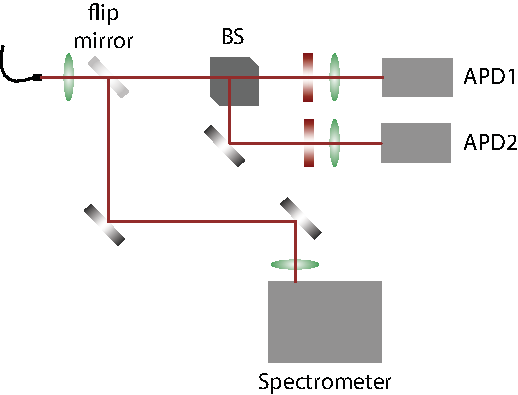
\includegraphics[trim = 0 0 0 0,  clip= true, width = 0.6\linewidth]{./pics/hbt_spectrometer.eps}}
			\caption[Spectrometer and HBT setup]{Spectrometer and HBT interferometer. Fluorescent light arrives via an optical fiber and is directed towards a flip mirror. The mirror directs the beam either towards a 50:50 beam splitter (BS) into the APDs of the HBT setup, or into a grating spectrometer.}
			\label{fig::hbt_spectrometer}
		\end{figure}

		In chapter \Fref{ch::coupling} we introduce applications of \sivs in \nds, for which knowing the precise positions of specific \nds is crucial.
		Therefore, cross markers are milled into the surface of the substrate on which the \nds are situated.
		These markers of a size of \SI{10}{\micro\meter} can easily be recognized by optical imaging and can thus be used as landmarks for the purpose of indexing individual \sivs.
		The starting point for a scan of an area of interest on the sample is fixed while navigating with the optical image.
		After flipping the flip mirror, light is directed towards the detection part of the setup enabling systematic scans of the sample.

	\section{Spectrometer} \label{sec::methods_spectrometer}

		\Fref{fig::hbt_spectrometer} displays the detection part of the setup.
		The \fl arrives via a pigtail fiber connecting the confocal setup with the detection setup and is out-coupled with an aspheric lens.
		A flip mirror is employed to direct the light either to a grating spectrometer or the \hbt setup.
		The optical spectrum of a light source gives insight to the optically active constituents and therefore bears information about the emitter.

		As mentioned before, the \fl from the \sivs is investigated with the grating spectrometer (Princeton Instruments Acton2500i).
		The incident beam passes through an entrance slit, is then scattered on the grating where the light is spectrally divided and finally hits a detector, imaging the entrance slit on the detector surface.
		The employed detector is a CCD camera (Princeton Instruments, Spec-10) cooled with liquid nitrogen to a temperature of \SI{-120}{\celsius}. This limits background signals due to thermally generated free charge carriers.
		The spectrometer is optimized for detection of light up to a \wl of \SI{900}{nm}.
		and features three gratings: \SI[per-mode=symbol]{600}{\lines\per\mm}, \SI[per-mode=symbol]{1200}{\lines\per\mm}, and \SI[per-mode=symbol]{1800}{\lines\per\mm}.
		These gratings are mounted on a turret, allowing easy swapping of gratings between measurements.

		With the spectrometer's step-and-glue function which is implemented in the spectrometer software (WinSpec) it is possible, to record several spectra over a wide \wl range which are then stitched together.
		It is therefore possible to combine a larger \wl range with a higher resolution.
		For most measurements the grating with \SI[per-mode=symbol]{600}{\lines\per\mm} was used.
		The resolution of the spectrometer using the \SI{600}{\lines\per\mm} is \SI{0.13}{nm} at \SI{738}{nm} and the accuracy amounts to \num{\pm0.4} as stated by the manufacturer.
		This resolution suffices for the measurements presented in this work.

	\section[HBT]{\HBT Setup}\label{sec::methods_hbt}

		A \HBT setup is used to establish the intensity autocorrelation function (\gt function) of an emitter \cite{brown1956correlation, brown1956test}.
		In this work, the \gtf is used to assert the non-classical behavior of a \pl source, \i.e.\ characterize its behavior as a single photon emitter.
		In the photon number representation, it is defined as follows:
		%
		\begin{equation}
		\gt(\tau) = \frac{ \mean{ N(t) N(t+\tau) } }{\mean{N(t)}^2}.
		\end{equation}

		Here, $N(t)$ denotes the number of photons at a certain time $t$, $N(t+\tau)$ denotes the number of photon at a time interval $\tau$ later than $t$.
		The angular brackets $\mean{}$ denote temporal averaging.
		For a two-level system $\gt(\tau)$ can be interpreted as the probability of detecting two photons separated by a time interval $\tau$.
		The physical intuition behind this definition is as follows: The detection of a fluorescent photon emitted from a quantum system is the result of an excited electron relaxing back to its ground state. To emit a consecutive single photon, an additional electron must first be promoted to an exited state, a process which takes a certain amount of time, see \Fref{ch::sivs}. If $\gt(\tau) \neq 0$ in the limit of $\tau \to 0$ a system is capable of emitting several photons simultaneously. This is known as photon bunching and is typical for classical light sources. In contrast, $\gt(\tau) \to 0$ for $\tau \to 0$ is an indication that no two photons can be detected simultaneously. This property is termed photon anti-bunching and is a defining characteristic of non-classical light sources such as \sps. The last important type are coherent photons, as for instance produced via stimulated emission. \Fref{fig::g2_illustration} shows how the \gt function distinguishes these three types. For an in-dept review of the intensity auto-correlation function we refer the reader to \cite{Neu2012, Fox2006}.

		\begin{figure}[!htb]
			\centering
			\testbox{\includegraphics[trim = 0 0 0 0,  clip= true, width = 0.6\linewidth]{./pics/g2_function_illustration.png}}
			\caption[Sketch of typical \gt functions]{Intensity autocorrelation function for coherent, bunched, and anti-bunched light sources. Figure and caption reproduced from \cite{rahbany2016towards}.}
			\label{fig::g2_illustration}
		\end{figure}


		The aim of the \hbt setup is to record the time delay between two consecutive photons as a prerequisite to compute $\gtz$.
		A sketch of the \hbt setup is shown in \Fref{fig::hbt_spectrometer}.
		Photons are detected using single photon \apds (\APDs, PicoQuant $\tau${}-SPAD100).
		\APDs are the semiconductor analog to photomultiplier tubes, i.e.\ an incoming photon creates secondary charge carriers through ionization.
		The secondary charge carrier is accelerated by a bias voltage to create further secondary charge carriers, resulting in an avalanche effect.
		Therefore, the signal of a single photon is intensified and detected as an electrical current pulse.
		These \apds have a nominal detection efficiency of up to \SI{70}{\percent} at an optimal wavelength of about \SI{670}{\nm} and a dark count rate of under \SI{100}{\cps}.
		If a charge carrier created by the avalanche is temporarily trapped and later liberated, it induces a so-called after-pulse.
		To avoid detecting these artifacts as real events, the \APDs have a dead time of about \SI{70}{\ns}.
		In the ideal case, one \APD would be enough to measure the time delay between two consecutive photons.
		However, the second of two consecutive photons could hit the detector during its dead time.
		To circumvent this problem, two \APDs are employed and the detection beam is split with a non-polarizing 50:50 beamsplitter cube.
		Each beam then goes through a band-pass filter and is focused on the \apd with an aspheric lens.
		As the beam path is slightly different for each \APD, a small optical path difference is introduced, however, this difference only results in an offset of the \gtf and does not alter the physical nature of the result.
		The bandpass filters serve two purposes:
		First, they limit optical crosstalk between the \apds.
		The detection process in an \apd produces light due to recombination of charge carriers.
		Crosstalk between two \apds occurs, if one of the photons produced by recombination in one \apd escapes and is detected in the other one \cite{Younger2009}.
		Second, the band-pass filters serve to reduce \bkg during the \gt measurement process or to spectrally separate emission from several emitters.
		Therefore, it is possible to find single emitters, which are not spatially separated enough to be separated by the spatial resolution of the setup.
		In particular, emitters can be individually investigated if their \ZPLs exhibit wavelengths which are spectrally well separated.
		Band-pass filters suited for the respective wavelengths are used to selectively investigate light associated with distinct \ZPLs.

		When the \APD fires, it outputs a digital TTL (transistor-transistor logic compatible) signal.
		The arrival times of the signals, so-called time-tags, are recorded with a time-tag unit (produced by dotfast-consulting) with a temporal resolution of \SI{78.125}{\pico\second}.
		The timing uncertainty of the photon detection process introduces variations of the digital signal's time-tag from the actual detection time.
		This is called timing jitter and adversely affects the recorded time-tags and consequently the value of $\gtz$. In the past it has been shown to significantly obfuscate the detection of anti-bunching behavior in \sps and thus relevant corrections need to be taken into account \cite{Neu2012, Riedrich-moller2014}.

		As stated earlier, the time delay between two consecutive photons is necessary for the reconstruction of the \gtf.
		The time delays are fed into a histogram which is then fitted to receive the continuous \gtf.
		As a suitable fit function a numerical convolution between the $\gt(\tau)$ derived for a three-level system and detector timing jitter can be used \cite{Neu2012b, Neu2012, Riedrich-moller2014}.

		In the \HBT{}-setup the arrival time of photons are recorded with two APDs, each of which keeping a list of arrival times as raw data.
		To get a single array of arrival times of the photons, which can then be binned to obtain the \gtf, the arrays of time-tags of the two \APDs have to be correlated.
		For that, the time difference between each entry in one array and all consecutive time-tags in the other array are determined and binned according to the timing resolution of the time-tag unit.
		After normalizing and fitting these data, \gtz can be obtained determining whether a emitter characterizes as a \sps.

  	%!TEX root = ../main.tex

\chapter{Experimental Results}	\label{ch::results}
\chaptermark{Results}

In the following paragraphs, both phenomenological of the nanodiamonds and spectroscopic measurement of the \sivs are described.
Unless explicitly otherwise stated, the results in this paper report measurements of the milled nanodiamonds containing \textit{in-situ} incorporated \sivs.

	%!TEX root = ../main.tex

\section{Diamond Characteristics}

	\subsection{Raman Measurements} \label{subsec::raman}



	%!TEX root = ../main.tex



\subsection[TEM]{Transmission Electron Microscopy} \label{subsec::tem}



	%!TEX root = ../../../main.tex



\section{Photoluminescence spectra} \label{subsec::spectra}


To find \nds containing \sivs on the substrate, confocal scans are performed.
The \sivs are further investigated by measuring \pl (PL) spectra, single photon statistics and photostability.
To reduce bias in the measurements, not only the brightest spots are investigated, but also those which are hardly brighter than \bkg fluorescence.
The luminescence spectrum of an \siv is composed of a prominent \zpl and weak sidebands.
Investigations of both are reported independently in the following paragraphs.



\subsection{\Zpl}\label{subsubsec::zpl}
	

	\begin{figure}[tp]
		\centering
		\testbox{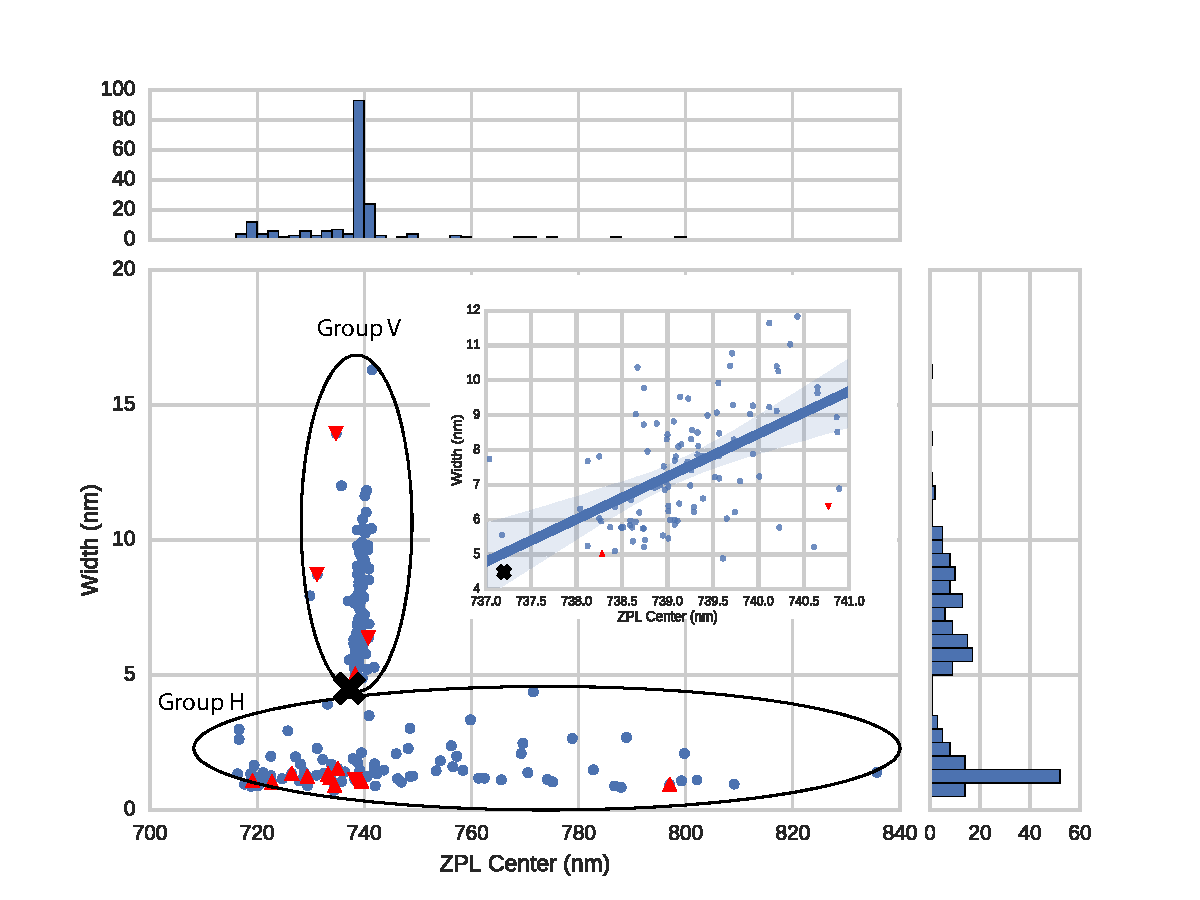
\includegraphics[trim = 0 0 0 0,  clip= true, width = 0.8\textwidth]{./pics/distro_histo_sarah_inset.pdf}}
		\caption{Distribution of the \lw vs. the center wavelength of the ZPL of the investigated \sivs in milled \nds containing \textit{in-situ} incorporated \sivs (samples \insituF, \insituS, \insituSn, \insituSo, \insituH{}). The data can be coarsely separated into two groups, H and V. The cross marks the position of an ideal \siv in unstrained bulk diamond \cite{Arend2016a}. The red triangles indicate emitters which exhibited an antibunching dip in the \gtz measurement. Upwards pointing triangles represent emitters which exhibit fluorescence intermittency (blinking), while triangles pointing down represent emitters which do not exhibit any blinking (see \autoref{subsec::photostab}). The inset displays a zoom into \vl, a least squares linear regression to the data, and the 95\% confidence interval of the regression as a shaded area around the fit line. A clear trend of broader \lws for longer \ZPL center shifts is visible.}
		\label{fig::bimodal_distr}
	\end{figure}


	\begin{figure}
		\begin{subfigure}[tp]{0.45\linewidth}
			\caption{}\label{subfig::emnarrow}
			\centering
			\testbox{\includegraphics[trim = 0 0 0 0 , clip = true, width = \linewidth]{./pics/Ir8_Spektrum_8_notitle.pdf}}
		\end{subfigure}
		\hfill
		\begin{subfigure}[tp]{0.45\linewidth}
			\caption{}\label{subfig::embroad}
			\centering
			\testbox{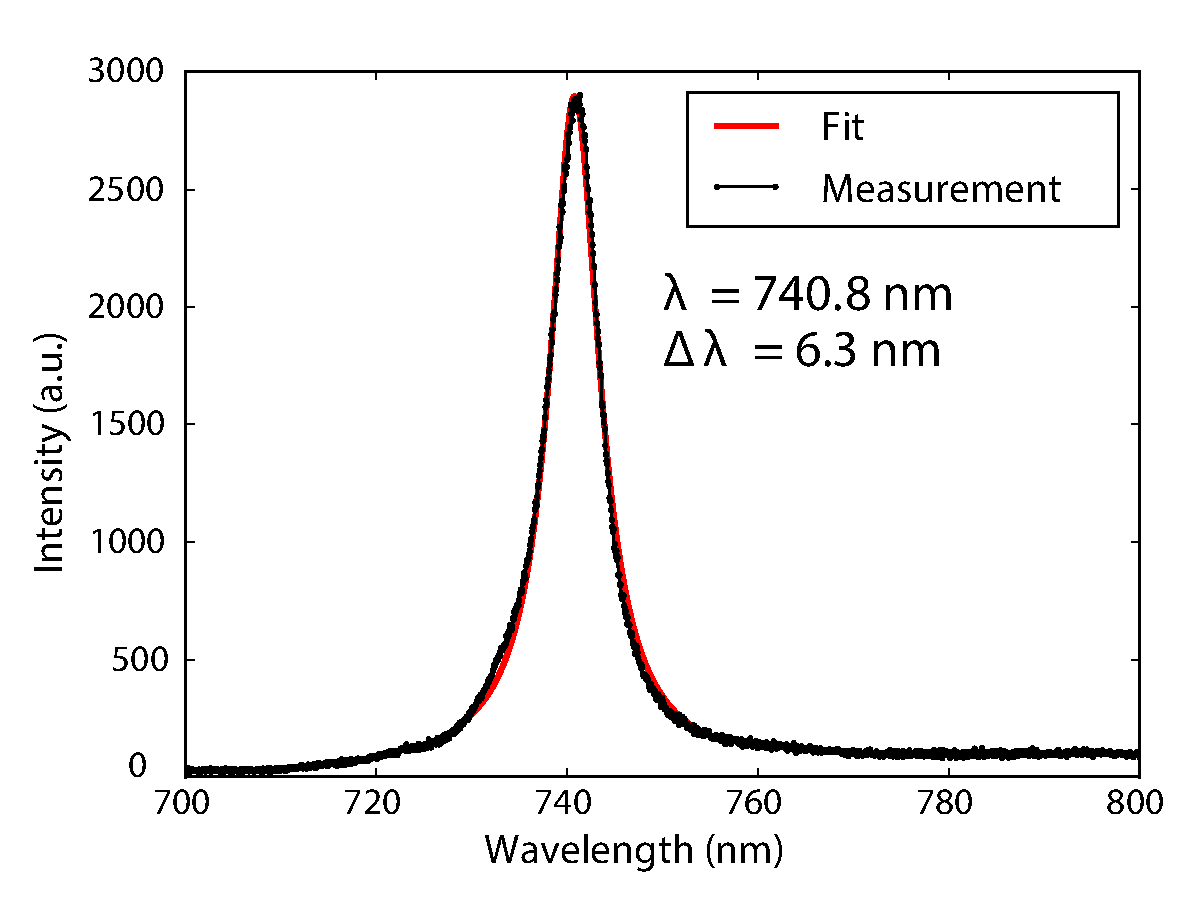
\includegraphics[trim = 0 0 0 0,  clip = true, width = \linewidth]{./pics/Ir8_scan_xy05_199uW_t30_notitle.pdf}}
		\end{subfigure}
		\caption{PL spectra measured with sample \insituHao. (a) A representative room temperature spectrum of one of the emitters in \hl of \autoref{fig::bimodal_distr}, denoted emitter \emnarrow. (b) A representative room temperature spectrum of one of the emitters in \vl of \autoref{fig::bimodal_distr}, denoted \embroad. The red lines are Lorentzian fits to the peaks.}
		\label{fig::spectra}
	\end{figure}

	\begin{figure}[tp]
		\begin{subfigure}[t]{ 0.49\linewidth}
			\centering
			\testbox{\includegraphics[trim = 0 0 0 0,  clip= true, width = \textwidth]{./pics/Ir22_spectrum_scan_xy01_x4y3_340uW_t30.pdf}}
			\caption{}
			\label{subfig::emnarrow2}
		\end{subfigure}
		\hfill
		\begin{subfigure}[t]{ 0.49\linewidth}
			\centering
			\testbox{\includegraphics[trim = 0 0 0 0,  clip= true, width = \textwidth]{./pics/Ir22_spectrum_scan_xy-40x81y323_392uW_t30.pdf}}
			\caption{}
			\label{subfig::embroad2}
		\end{subfigure}
		\caption{Other representative examples for a) a narrow and b) a broad \ZPL}
		\label{fig::spectra2}
	\end{figure}

	\begin{figure}[tp]
		\centering
		\testbox{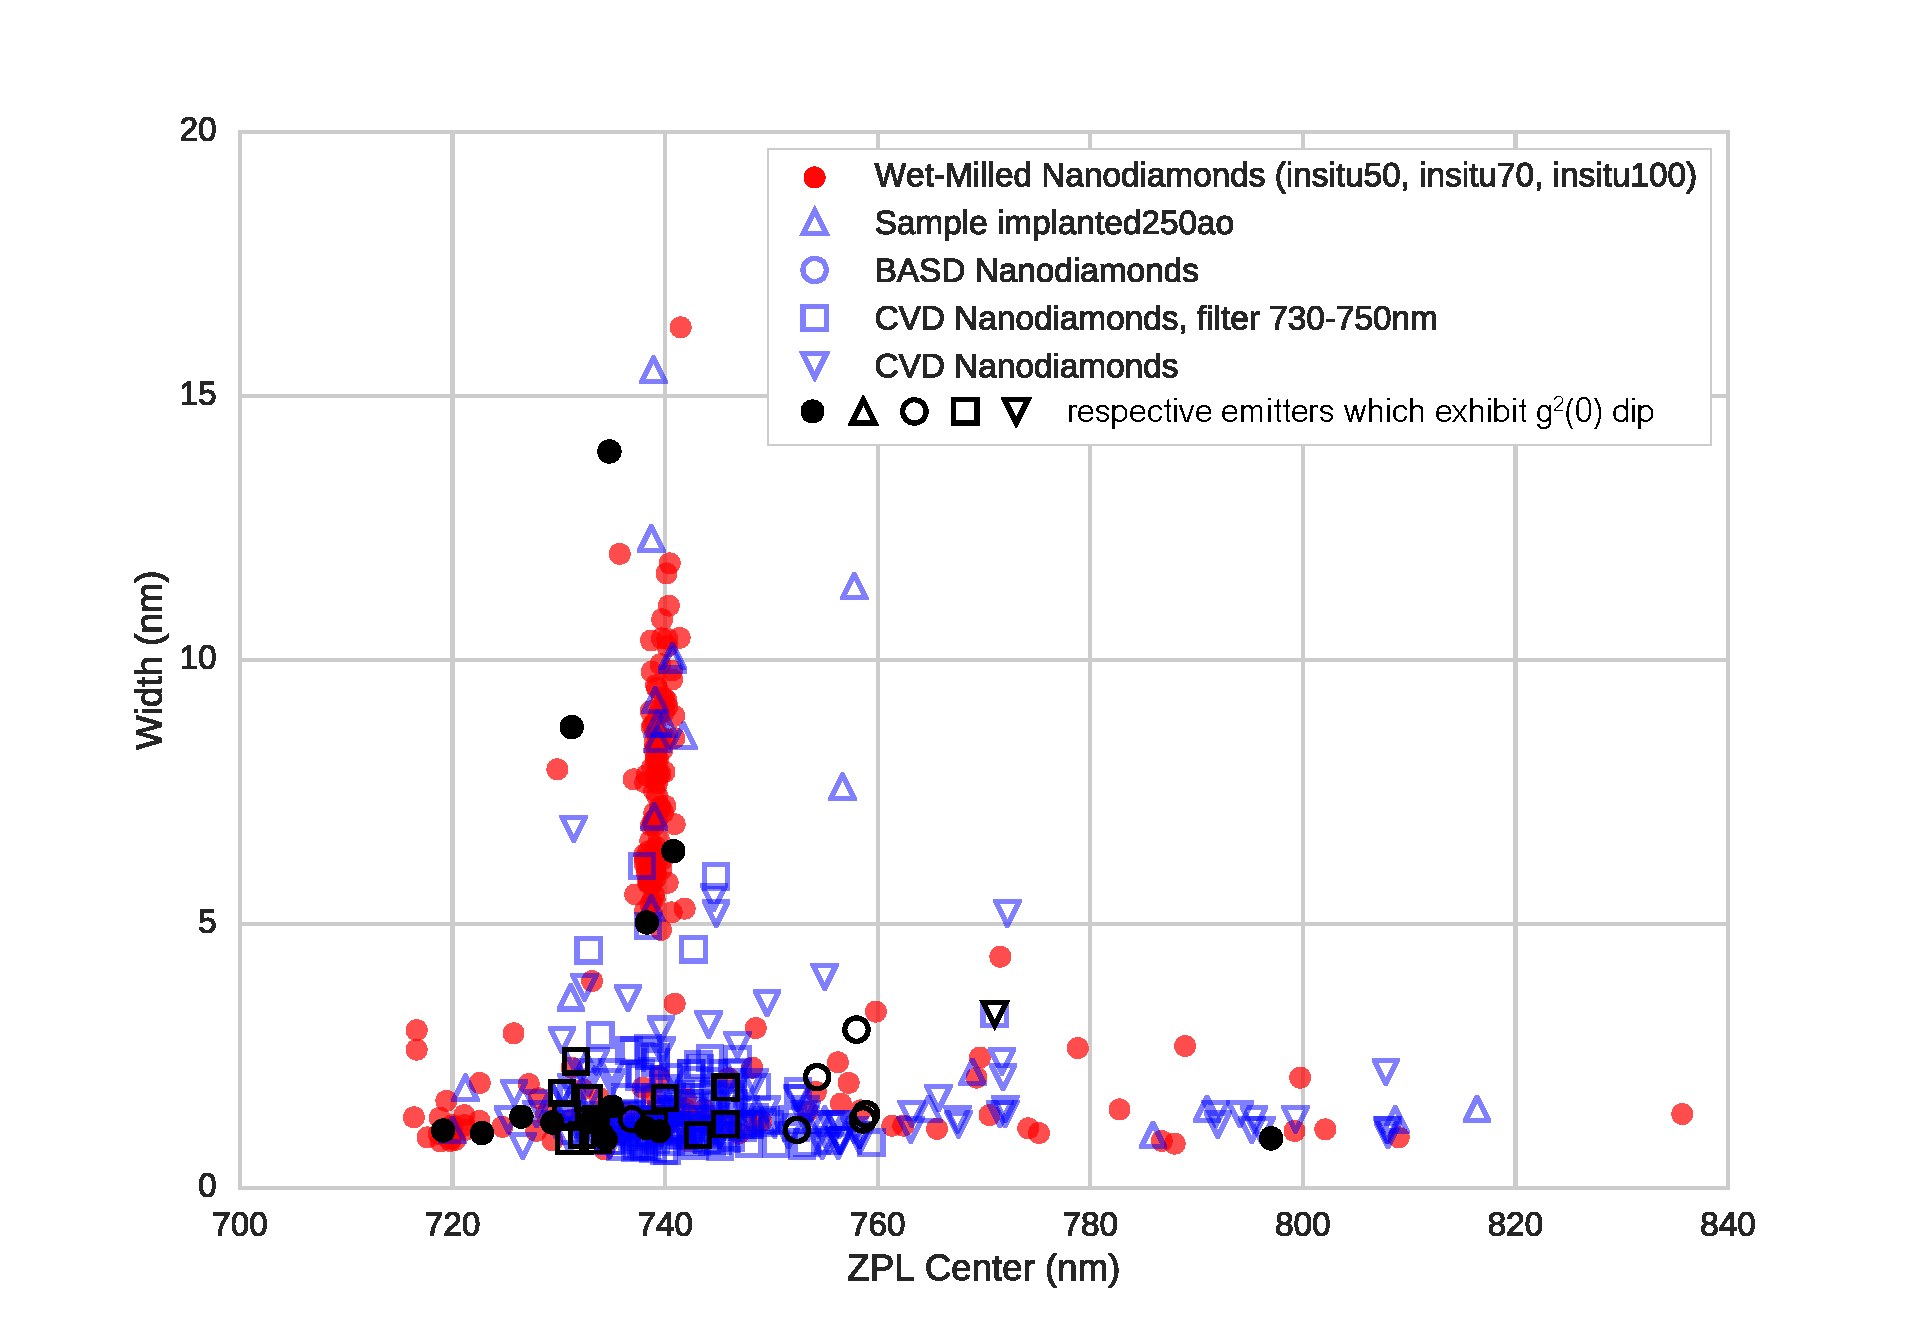
\includegraphics[trim = 0 0 0 0,  clip= true, width = 0.7\textwidth]{./pics/red_blue_markers_in_legend.pdf}}
		\caption{Comparison of the distribution of the \lw vs. the center wavelength of the ZPL of the investigated \sivs in milled \nds with data measured on the same \nds reported by J. Benedikter in \cite{Benedikter2017a}, with data measured on CVD \nds, with data measured in CVD diamonds by E. Neu in a filter window between \SIlist{730; 750}{nm} \cite{Neu2012}, and with data measured on \implantedTao, implanted with \Si. Black symbols represent emitters exhibiting a dip in the \gtz function, indicating a single or very few \sivs}
		\label{fig::bimodal_distr_compare}
	\end{figure}

	\begin{figure}[tp]
		\centering
		\testbox{\includegraphics[trim = 0 0 0 0,  clip= true, width = 0.5\textwidth]{./pics/ZPL_shift_SiV_new.pdf}}
		\caption{Calculations of the wavelength of the \siv \ZPL in dependence of pressure. Black: hydrostatic pressure; other colors: uniaxial pressure, for different orientations and calculated with different functionals PBE and HSE. Hydrostatic-type pressure causes a moderate blue shift whereas uniaxial strain causes larger redshift with different magnitudes depending on the direction of the strain \correct{better description from Adam Gali}}
		\label{fig::stress_pressure}
	\end{figure}


	The \cwl and the \lw of the \zpl of each measured SiV luminescence spectrum of the samples \insituF, \insituS, and \insituH are determined by fitting a Lorentzian fit to the \ZPL.
	Both spectra from single and multiple \sivs are taken into account.
	The \lw of each ZPL is plotted against its \cwl (\autoref{fig::bimodal_distr}).
	What immediately strikes the eye is a pattern that to our knowledge has not been reported to date: 
	The observed ZPLs accumulate in two different regimes, namely a horizontal lobe (denoted \hl) and a vertical lobe (\vl) divided by a gap with hardly any data points. 
	Single emitters are found both in \hl and \vl (for more details about single emitters see section \ref{subsec::g2}).
	\\
	The two groups are defined by their characteristic \cwls and \lws: 
	In \hl very prominent ZPL peaks are found which show \lws between about \SIrange{1}{5}{nm} at \cwls which vary between about \SIrange{715}{835}{nm}.
	\autoref{subfig::emnarrow} shows a representative spectrum of a single emitter of \hl (denoted \emnarrow), exhibiting a ZPL line width of \SI{1.4}{nm} at a \cwl of \SI{726.5}{nm}.
	In contrast, in \vl, the spectra exhibit broader ZPL \lws of about \SI{5}{nm} up to \SI{18}{nm}.
	Their ZPL \cwls, however, are distributed within a very narrow range between \SIrange{738}{741}{nm}.
	\autoref{subfig::embroad} shows a spectrum of a single emitter of \vl (denoted \embroad), exhibiting a ZPL \lw of \SI{6.4}{nm} at a \cwl of \SI{740.8}{nm}.
	For comparison, the room temperature ZPL of \sivs in unstrained bulk diamond shows a \lw of \SIrange{4}{5}{nm} at a \cwl of \SI{737.2}{nm} marked with a cross in \autoref{fig::bimodal_distr} \cite{Arend2016a,Dietrich2014}. 
	\\
	We also investigated the \db of the reported spectra, which states the amount of emission light stemming from the \ZPL wrt. emission from sidebands.
	The \db of \emnarrow  amounts to \num[separate-uncertainty]{0.81(1)}, corresponding to a \hr factor of \num[separate-uncertainty]{0.21(1)} which is in good agreement with the values reported in \cite{Neu2011b}.
	The error is mainly due to background correction. 
	When zooming in to the spectrum of \embroad it shows, that it does not exhibit any sidebands, i.e. all emission goes into the ZPL. 
	Considering resolution limits of the spectrometer, the \db factor amounts to close to 100\%.
	The signal-to-noise ratio in the chosen spectral window amounts to $93\%\pm1\%$.
	It has to be pointed out, that we did not find any systematic difference of the \db factor between \hl and \vl.
	\\
	As the broad \ZPL distribution shown in \autoref{fig::bimodal_distr} is unreported so far, we compare the results both to previous measurements and a control sample fabricated by \si implantation.
	The comparison of current, earlier and control data is presented in \autoref{fig::bimodal_distr_compare}.
	Samples for which previous data has been taken are:
	\begin{enumerate}
		\item \nds produced by \basd (BASD) of polycrystalline \CVD diamond films (\cite{Neu2011a}; data taken from \cite{Benedikter2017a})
		\item \nds produced directly via a \CVD process with \textit{in-situ} incorporated \sivs; measured in a spectral filter window of \SIrange{730}{750}{nm} (data reused from \cite{Neu2012} with permission)
		\item \nds produced in the same manner as the sample above; spectroscopic measurement procedure the same as the one performed on the milled, \textit{in-situ} implanted samples (see \autoref{tab::samplenames}, \insituF etc.)
	\end{enumerate}
	All previous data from different \nd material fit nicely with the \ZPL distribution.
	To rule out that the two lobes in the distribution are no artifacts due to other elements incorporated into the \nds during the process, such as residue from other processes performed in the growth chamber or material abrasion from chamber parts and to verify that the observed luminescent defects are indeed \si related, we performed control experiments that were implanted with \si to form \sivs (sample \implantedTao).
	\autoref{fig::bimodal_distr_compare} shows that the implanted \sivs cover roughly the same spectral range as the grown-in centers, thereby providing strong evidence for the \si related origin of the defects.
	\\
	In the next paragraphs, the \ZPL distribution will be discussed in further detail.
	At first, the \ZPL \cwl shift is investigated.
	Very few of the measured data points in \vl sit at a shorter \cwl than the point attributed to an ideal \siv in unstrained bulk material.
	This means, a red-shift of the \ZPL of an \siv is more likely than a blueshift.
	Several mechanisms contribute to the \cwl shift, namely hydrostatic- and material strain.
	As explained in \autoref{subsec::raman}, we measured the Raman shift of samples \insituS and \implantedTao.
	These measurements indicate strain in the diamond lattice.
	\autoref{fig::stress_pressure} shows the calculated shift of the  \ZPL in dependence of pressure in the diamond lattice both for hydrostatic stress and for uniaxial stress.
	PBE and HSE are two different funtionals used for the calculations \todo{input Adam Gali}.
	From \autoref{fig::stress_pressure} it can be seen, the assumption stated in \autoref{subsec::raman} that the strain in the \nds is mainly due to uniaxial stress corresponds well with the measured \ZPL red-shift in \vl.
	With higher uniaxial pressure, the \ZPL becomes more and more red-shifted.
	However, the measured shifts in \hl are too broad to be solely explained by strain in the diamond.
	We suspect that there are other defect sites present in the vicinity of the \siv which explain the strong variation \cite{Thiering2015}.
	This statement is strengthened by the measurement of the shift of the first order Raman peak to lower wavenumbers.
	The investigation of this hypothesis presents an interesting topic for further research.
	\\
	Zooming in to \vl, another effect becomes visible (inset in \autoref{fig::bimodal_distr}):
	With increasing  \ZPL, the \lw becomes broader.
	The data points in \vl are fitted with a linear regression to guide to the eye.
	Linking the correspondence between the strain and the red-shift of the \ZPL with that of the slope of between the \cwl of the \ZPL and the \lw leads to the conclusion that also the \lw is affected by strain in the diamond lattice: The higher the uniaxial stress, the bigger the linewidth.
	\\
	To conclude, we are able to explain \vl very consistently with theoretical predictions for the \ZPL \cwl shift due to strain in the diamond lattice. 
	On the other hand, we suspect that \hl is due to lattice defects in the vicinity of the \siv, which has to be investigated in further research.

	%!TEX root = ../../../main.tex

	\subsection{Sideband} \label{subsubsec::sideband}

		It is known that the \pl spectra of \sivs in \nd are dominated by the \zpl. As a result \psb contributions remain small, a fact expressed in large \db factors of over \SI{70}{\percent} established previously \cite{Neu2011,Neu2011b}. Our own measurements are consistent with these of \emnarrow and \embroad results. We also find distinct sideband peaks in many \siv \pl emission spectra.
		The investigated emitters exhibit two different structures of sideband spectra: The spectra in \vl exhibit one strong sideband peak, spectra in \hl exhibit several weaker sideband peaks. \Fref{subfig::sideband_group_v} and \Fref{subfig::sideband_group_h} illustrate the respective observations.

		\begin{figure}[!htb]
			\begin{subfigure}{0.49\linewidth}
				\centering
				\testbox{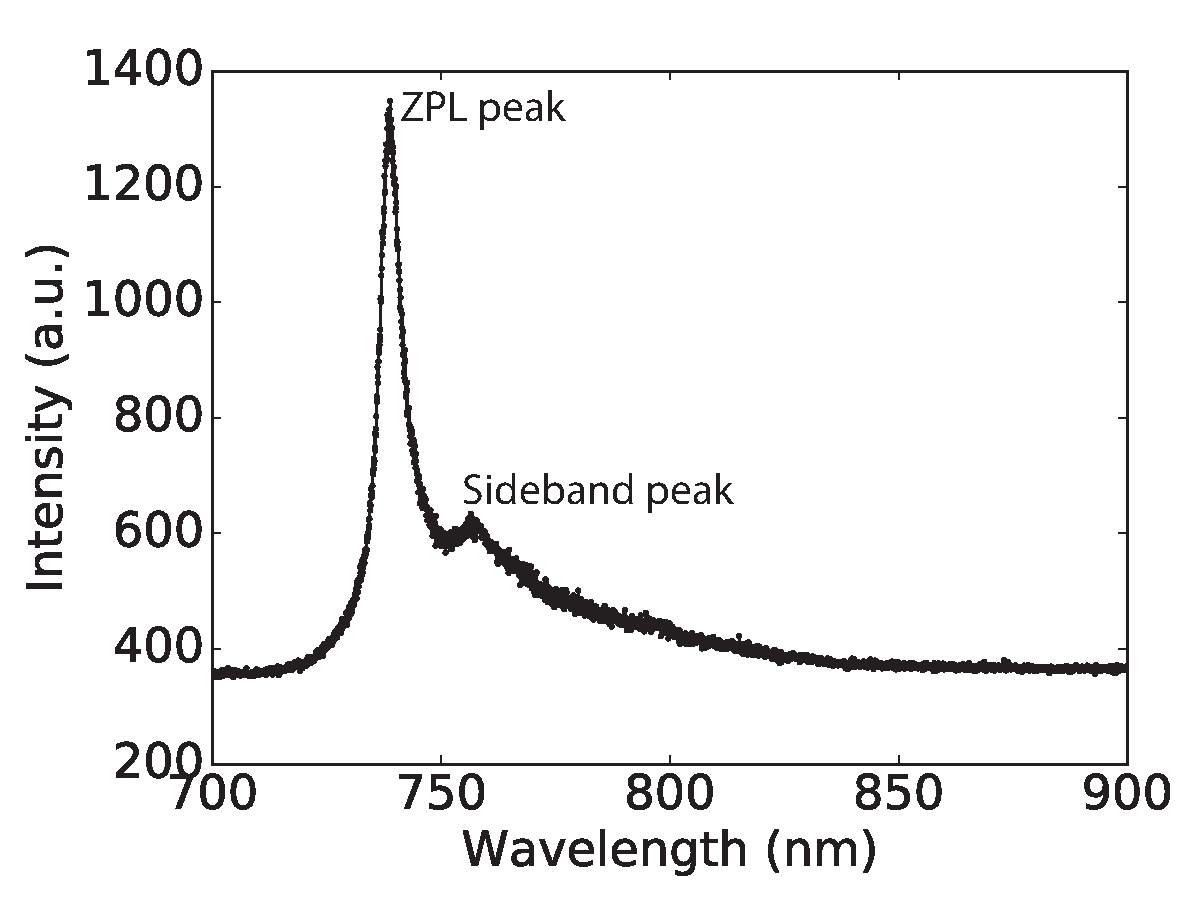
\includegraphics[trim = 0 0 0 0,  clip= true, width = \pairplotwide]{./pics/Ir25M_spe_scan_xy-38x9y16_300uW_t120.pdf}}
				\caption{}
				\label{subfig::sideband_group_v}
			\end{subfigure}
			\hfill
			\begin{subfigure}{0.49\linewidth}
				\centering
				\testbox{\includegraphics[trim = 0 0 0 0,  clip= true, width = \pairplotwide]{./pics/G4_9_30s.png}}
				\caption{}
				\label{subfig::sideband_group_h}
			\end{subfigure}
			\caption[Side band peaks for \sivs]{Representative spectra of emitters showing single (\subref{subfig::sideband_group_v}) and multiple (\subref{subfig::sideband_group_h}) side band peaks. The former belong to \vl, while the latter are members of \hl.}
			\label{fig::sideband_groups}
		\end{figure}

		Most of the spectra in \vl exhibit a characteristic shape, composed of the \ZPL and one strong sideband peak.
		\SI{70}{\percent} of the \pl spectra with one distinct sideband peak exhibit a shift of the sideband peak from the \ZPL between \SIrange{37}{43}{meV}.
		The range of line shifts for the prominent sideband peak coincides with a well-known feature at \SI{42}{meV}, associated with \sivs \cite{Larkins1971,Sternschulte1994}, but also to a larger number of optically active defects \cite{Sternschulte1994}.
		The occurrence of this \SI{42}{meV} sideband feature for a large number of defects and the absence of isotopic variations \cite{Dietrich2014}, favors an assignment as non-localized lattice vibration.
		We furthermore observe that the dominant sideband peak shifts towards smaller distance from the \ZPL for increasing \ZPL \cwl, i.e.\ increasing strain. \Fref{fig::sideband_fit} presents a linear fit to data for emitters in \vl..
		The low phonon energy of the sideband feature and its shift with strain might arise from a local ``softening'' of the crystal lattice in the vicinity of a defect \cite{Sternschulte1994}.

		\begin{figure}[!htb]
			\centering
			\testbox{\includegraphics[trim = 0 0 0 0,  clip= true, width = 0.6\linewidth]{./pics/sideband_regression.pdf}}
			\caption[Shift of dominant side band peaks for \sivs]{Shift of dominant sideband peak from the \ZPL in spectra of \sivs (\vl, samples \insituF, \insituS, \insituH) vs. ZPL \cwl. The linear fit shows that the shift decreases with increasing ZPL center wavelength, i.e.\ with increasing strain and exhibits a slope of \SI[separate-uncertainty]{-4\pm1}{\milli\electronvolt\per\nano\meter}. The shaded area is the \SI{95}{\percent} confidence region.}
			\label{fig::sideband_fit}
		\end{figure}

		A recent study \cite{Londero2016} suggests that the \SI{42}{meV} mode, similar to other broad \psb features, originates from a resonance attributed to phonons causing the dynamical Jahn-Teller effect with \sivs \cite{Fu2009}.
		As the Jahn-Teller coupling varies with strain it is also expected that the resonance shifts accordingly.
		\\
		In the spectra of \vl, we do not observe a typical \siv sideband feature at \SI{64}{meV}, attributed to a local vibration of the \si atom, frequently much stronger than the  \SI{42}{meV} sideband peak.
		A possible explanation is, that the lattice mode at \SIrange{37}{43}{meV} is so strong that the local vibrational mode at \SI{64}{meV} cannot be separated from the tail of the lattice mode.
		% \\
		% \todo{beginning new}For further investigations, we plotted the \ZPL  of \vl with multiple peaks.
		% We found that two Lorentzian curves fit the peak best.
		% \Fref{fig::sideband_multfit} shows histograms of the distribution of the \cw and the \lw of the fitted peaks.
		% Keep in mind that two of the peaks sum up to the peak visible as a \ZPL and the third peak is the sideband peak which we attribute to the lattice mode at about \SI{43}{meV}.
		% We found that the \lw of the sideband peak exhibits values up to \SI{20}{nm}.
		% This broad width is an indicator, that the local vibrational mode might indeed be outpowered by the more intense lattice mode.
		% However, it is not very easy to find spectra where the sideband peak is pronounced and isolated enough to make proper statistics.
		% The original \ZPL is split up in two peaks, one with a median \cwl of \SI{738}{nm} (\SI{1680}{\meV}) and a median \lw of \SI{4.5}{nm}  and the other with a median \cwl of \SI{742}{nm} (\SI{1671}{\meV}) and a median \lw of \SI{8}{nm}.
		% It could be that this is an indication for another sideband peak with a shift of \SI{9}{\meV}.
		% \todo{end new}
		% \\
		% \begin{figure}[tp]
		% 	\begin{subfigure}[t]{ 0.49\linewidth}
		% 		\centering
		% 		\testbox{\includegraphics[trim = 0 0 0 0,  clip= true, width = \textwidth]{./pics/histo_multi_sidebands_position25bins.pdf}}
		% 		\caption{}
		% 		\label{subfig::sb_multfit_pos}
		% 	\end{subfigure}
		% 	\hfill
		% 	\begin{subfigure}[t]{ 0.49\linewidth}
		% 		\centering
		% 		\testbox{\includegraphics[trim = 0 0 0 0,  clip= true, width = \textwidth]{./pics/histo_multi_sidebands_width_25bins.pdf}}
		% 		\caption{}
		% 		\label{subfig::sb_multfit_width}
		% 	\end{subfigure}
		% 	\caption{}
		% 	\label{fig::sideband_multfit}
		% \end{figure}
		% \\
		In \hl we observe many spectra which exhibit several peaks within the spectral range of our detection range between \SIrange{710}{900}{nm}.
		The challenge arises to unequivocally distinguish between peaks stemming from a phonon sideband and peaks stemming from shifted, less intense \siv \ZPLs.

		Interestingly, we assert a tendency for peaks to accumulate at a shift of around \SIlist{43;64;150;175}{meV}, as shown in \Fref{fig::multiple_sb_peaks}. This pattern in the \psb of \hl is consistent with side band shifts reported in \cite{Sternschulte1994,Zaitsev2000, Neu2011}.

		\begin{figure}[!htb]
			\centering
			\testbox{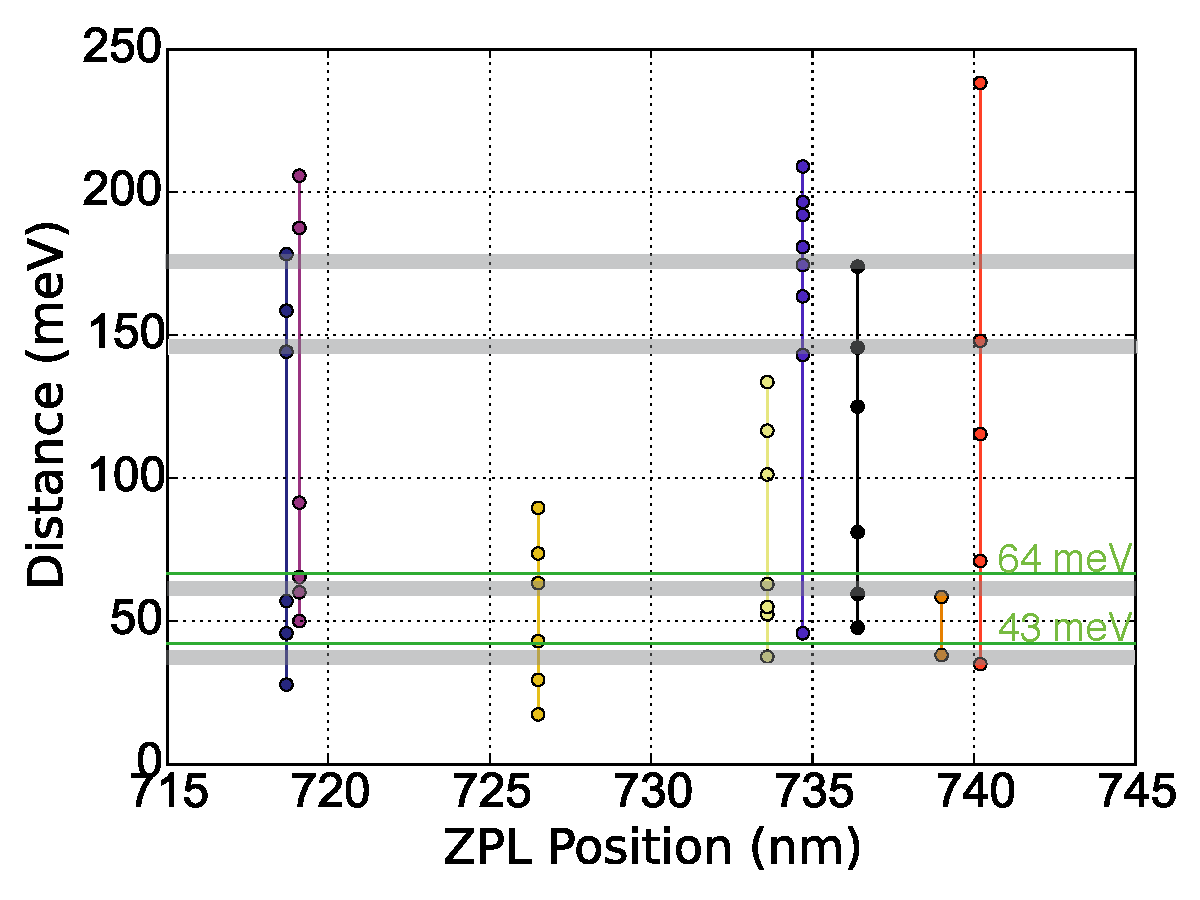
\includegraphics[trim = 0 0 0 0,  clip= true, width = 0.6\linewidth]{./pics/statistics_only_multiple_sb_zpl_vs_distance_5meVbars_modes_edit.png}}
			\caption[Accumulation of sideband peaks]{This plots shows sideband peaks attributed to different \ZPL \cwls, with respect to the sideband peak's shift. The \ZPL \cwl is visualized on the x-axis, the respective sideband peak shifts on the y-axis. Therefore, data points aligned on a vertical line belong to the same spectrum. For better visibility, all data points of one spectrum are colored in the same color. Areas shaded in grey represent an accumulation of sideband shifts. The green lines indicate distances with \SI{43}{meV} and \SI{64}{meV} respectively.}
			\label{fig::multiple_sb_peaks}
		\end{figure}

		The possibility exists, that some these peaks believed to be \psbs are actually shifted \ZPLs stemming from other \sivs. To address this question, we perform \pl measurements at cryogenic temperatures.


		\subsection{Cryostatic Measurements}\label{subsec::cryo}

			\begin{figure}[!htb]
				\begin{subfigure}[t]{ 0.49\linewidth}
					\centering
					\testbox{\includegraphics[trim = 0 0 0 0,  clip= true, width = \pairplotwide]{./pics/Ir25Mox_fit_spe_scan_xy-08x11y19_297uW_t180.png}}
					\caption{}
					\label{subfig::roomtep1}
				\end{subfigure}
				\hfill
				\begin{subfigure}[t]{ 0.49\linewidth}
					\centering
					\testbox{\includegraphics[trim = 0 0 0 0,  clip= true, width = \pairplotwide]{./pics/cryo_Spektrum68_edit.png}}
					\caption{}
					\label{subfig::cryo1}
				\end{subfigure}
				\hfill
				\begin{subfigure}[t]{ 0.49\linewidth}
					\centering
					\testbox{\includegraphics[trim = 0 0 0 0,  clip= true, width = \pairplotwide]{./pics/Ir25M_rt_to_cryo_84_fit_spe_scan_xy-35x10y12_300uW_t120.png}}
					\caption{}
					\label{subfig::roomtep2}
				\end{subfigure}
				\hfill
				\begin{subfigure}[t]{ 0.49\linewidth}
					\centering
					\testbox{\includegraphics[trim = 0 0 0 0,  clip= true, width = \pairplotwide]{./pics/cryo_Spektrum84_edit.png}}
					\caption{}
					\label{subfig::cryo2}
				\end{subfigure}
				\caption[Spectra of \nds at cryogenic temperatures]{Comparison of spectra taken at room-temperature (l.h.s) and at cryogenic temperatures (r.h.s). At low temperatures a multitude of lines is revealed indicating several \sivs embedded in a strained lattice neighborhood.}
				\label{fig::rt_vs_cryo}
			\end{figure}

			At cryogenic temperatures \psb contributions vanish, allowing a focused investigation of \zpls.
			In particular, for \sivs a four-way splitting of the \zpl is expected, see \Fref{ch::introduction}.
			To conduct low-temperature measurements, we used a confocal setup similar to the one described in \Fref{ch::pl_setup}.
			It differs merely by the fact that the sample is efficiently cooled to \SI{4}{\kelvin} using a cryostat.
			\\
			In \Fref{fig::rt_vs_cryo} measurements of two individual \nds are shown, both situated on sample \insituSo.
			\Fref{subfig::cryo1} and \Fref{subfig::cryo2} show spectra recorded at cryogenic temperatures while \Fref{subfig::roomtep1} and \Fref{subfig::roomtep2} show spectra recorded at room temperature for comparison.
			Instead of the four-fold degeneracy expected for \sivs in low-strain diamond, the cryogenic measurements indicate a multitude of various lines.
			The observation is best explained by the presence of several \sivs which are subject to varying levels of strain in their local lattice neighborhood.
			Given the fact that \zpls are found spread over a significant range of \wls, a non-negligible impact of lattice strain on \siv luminescence is revealed.

	%!TEX root = ../main.tex




\section{Photon correlation measurements} \label{sec::g2}


	%!TEX root = ../main.tex




	\section{Photostability} \label{sec::photostab}


  	%!TEX root = ../main.tex


 \chapter{discussion}	\label{ch::discussion}
  	%!TEX root = ../../main.tex


 \chapter*{Summary and Conclusions}	\label{ch::conclusion}
 \addcontentsline{toc}{chapter}{Summary and Conclusions}
   % short summary of what happened in the thesis

   % important stuff from siv paper

   In conclusion we found a strongly inhomogeneous distribution of \siv spectra in nanodiamonds.
   We group the \zpls into two groups:
   \Hl consists of \ZPLs exhibiting a narrow \lw from below \SI{1}{nm} up to \SI{4}{nm} and a broad distribution of \cwl between \SIlist{710;840}{nm}.
   Compared to that, \vl comprises \ZPLs with a broad \lw between just below \SIlist{5; 17}{nm} and \cwl ranging from \SIrange{730}{742}{nm}.
   This data is consistent with previously measured SiV spectra \cite{Benedikter2017a,Neu2012}.
   For comparison, an \siv in unstrained bulk diamond exhibits a \lw of \SIrange{4}{5}{nm} at a center wavelength of \SI{737.2}{nm}\cite{Arend2016a,Dietrich2014}.
   We show that both the observed blue-shift and the observed red-shift of \vl are consistently explained by strain in the diamond lattice.
   Further, we suggest, that \hl might be comprised of modified \sivs, the structure of which is currently unclear.
   \\
   We investigated the SiV sidebands:
   In \vl we found one prominent peak at a shift of \SI{42}{meV}, which corresponds to a well-known feature assigned to non-localized lattice vibrations \cite{Larkins1971,Sternschulte1994}.
   In \hl we see an accumulation of peaks, at around \SIlist{43;64;150;175}{meV}, which are consistent with sideband peaks reported in \cite{Sternschulte1994,Zaitsev2001,Neu2011}.
   \\
   We further reported photon autocorrelation measurements which verified the existence of single \sivs both in \hl and \vl.
   Investigating the time trace of the \siv \pl, we found that some \sivs exhibit fluorescence intermittence with on times between several microseconds up to \SI{41}{s}.
   Furthermore, we see an exponential distribution of bright time intervals and a log-normal distribution of dark time intervals, consistent with research on single molecules \cite{Wong2013}.
   In terms of photostability, there is a big difference between \vl and \hl:
   All but one emitters in \hl exhibit blinking, where only one of the emitters in \vl exhibits blinking.


   % important facts from coupling chapter

   To effectivly quantify the emission enhancement provided by the plasmonic double bowtie antenna, a single \siv is necessary.
   A correct measure for the emission enhancement is the saturation count rate since it is proportional to the inverse of the emitter's lifetime.
   Hence, if there are two or more emitters present, photons of the individual emitters are emitted randomly, which renders a correct saturation measurement impossible.
   However, finding \sivs in \nds which fulfill both spectroscopic (\gtz $\approx$0, saturation, narrow \ZPL spectrum) and technical (size, isolation of \nds) constraints is an extremely time-consuming process. It is a search for the needle in the haystack.
   \\
   We investigated different kinds of \nds in the search of \nds exhibiting optimal spectroscopic and technical parameters.
   We were able to fulfill the size requirements posed by the \pp process and antenna design by producing different patches of different sizes of \nds and took the ones which were best suited.
   We also developped a good isolation of the \nds on the substrate by treating the \ir substrate with Piranha etch and tuning the amount of diamond solution drop-casted onto the substrate.
   This leaves us with the need of a higher propability of exactly one \siv per \nd.
   Parameters which have an impact on the quantity of \sivs per \nd are the initial \siv density in the starting material and the \nd size.
   Once the time constraint of finding a single \siv in a \nd is overcome, we can apply the extensive methods and knowledge gained by the reported procedures to couple a single \siv to a plasmonic bowtie antenna.
   \\
   To our knowledge, our experiments were the first attempts of coupling \sivs to plasmonic bowtie antennas.
   The extraordinarily precise correlation of the theoretically predicted and the experimentally recorded spectrum of an ensemble of \sivs in a \nd make this process a promising candidate for future applications.


   % establishing connection to introduction and quantum candela

   adding momentum towards the adoption of the quantum candela \dots

	%!TEX root = ../main.tex


\appendix

    %!TEX root = ../main.tex

\chapter{Text of Minor Interest} \label{app::A}





			\label{appendices}	
	%!TEX root = ../main.tex

  \cleardoublepage
  \phantomsection
  \addcontentsline{toc}{chapter}{\bibname}
%   \bibliographystyle{abbrv}
    \bibliographystyle{unsrt}
  \bibliography{./bibliography/library}



 

 		\label{bibliography}	
	
% 	\cleardoublepage
	\phantomsection
	\addcontentsline{toc}{chapter}{\indexname}
	\printindex					\label{index}
	
\end{document}